% !TEX root = main.tex
\chapter{Data sample and selection}

This analysis is done on the data sample recorded by the \lhcb experiment in \num{2011} and \num{2012} at centre-of-mass energies of \SI{7}{\tera\electronvolt} and \SI{8}{\tera\electronvolt}, respectively.
In \num{2011} the detector collected \SI{1}{\per\femto\barn}, while in \num{2012} \SI{2}{\per\femto\barn} were collected.
In this chapter first the used data samples as well as the simulated samples are described (\cref{sec:Samples}).
Following the selection procedure is reported, divided into preselection and trigger requirements (\cref{sec:preselTrigger}), vetoes for \eg misidentified background events (\cref{sec:vetoes}) and a multivariate classifier to reduce combinatorial background (\cref{sec:MVADev} and \cref{sec:BDTOpt}).
Last the handling of multiple $B$-candidates in one event is presented (\cref{sec:MultCands}) and the selection performance is given (\cref{sec:selectionPerformance}).

\section{Data and simulation samples}
\label{sec:Samples}

Candidates for the decay \BdToDpi are reconstructed in the hadronic decay $\Dpm\!\to\Kmp\pipm\pipm$ with one additional pion, which will be denoted as bachelor pion in the following.
Since the \D-decay is the one with the largest decay width it is chosen, despite the purely hadronic final state.
It is reconstructed inclusively, \ie no resonances as the decay via a \Kstarz are excluded.

To distinguish the charged hadrons in the finalstate a likelihood function assuming the respective particle to be a pion or a kaon is computed for every particle using information from the PID system.
The difference between the two logarithmic likelihoods is then calculated, referred to as \dllkpi in the following.
To identify other particles like protons a likelihhod function assuming a hypothesis can be computed and compared in the same way to the pion hypothesis.
Using the \dllkpi of the bachelor pion allows to split the data sample in two parts: The first sample denoted as \emph{pion}-sample with $\dllkpi\leq5.0$ and a second sample denoted as \emph{kaon}-sample with $\dllkpi>5.0$. This distinction is useful when separating \BdToDpi candidates from $\Bd\!\to\Dm\Kp$ candidates as no dedicated selection cut is needed, but instead this separation can be done statistically in the fit to the invariant mass distribution.

The simulated samples which were used in this analysis are listed in \cref{tab:simSamples}, together with short reference in which step they were needed (charge conjugation is implied throughout the whole document if not stated otherwise).
\begin{table}[tbp]
	\centering
	\caption{Simulated samples used in this analysis with a short note in which analysis step the samples were used. Charged \D-mesons are always generated with the decay $\Dm\!\to\Kp\pim\pim$, uncharged \D-mesons with the decay $\Dzb\!\to\Kp\pim$.}
	\begin{tabular}{lc}
		\toprule
		sample & analysis step \\
		\midrule
		$\Bz\!\to\Dpm\pimp$ 														& selection, massfit, flavour tagging, time fit \\
		$\Bs\!\to\Dsm\!\left(\to\Kp\Kp\pim\right)\pip$  							& selection \\
		$\Lb\!\to\Lcbar\!\left(\to\Kp\antiproton\pim\right)\pip$ 					& selection \\
		$\Bz\!\to\Dm\Kp$ 															& massfit \\
		$\Bz\!\to\Dm\rhop\!\left(\to\pip\piz\!\left(\to\g\g\right)\right)$ 			& massfit \\
		$\Bz\!\to\Dstarm\!\left(\to\Dm\piz\right)\pip$ 								& massfit \\
		$\Bz\!\to\Dm\Kstarp\!\left(\to\Kp\piz\right)$ 								& massfit \\
		$\Bz\!\to\jpsi\!\left(\to\mup\mun\right)\Kstarz\!\left(\to\Kp\pim\right)$ 	& flavour tagging \\
		$\Bu\!\to\Dzb\pip$ 															& flavour tagging \\
		$\Bu\!\to\Dzb\Kstarp\!\left(\to\Kp\pim\right)$ 								& flavour tagging \\
		$\Bu\!\to\Dstarb\!\left(\to\Dz\g\right)\pip$ 								& flavour tagging \\
		$\Bu\!\to\Dzb\Kstarp\!\left(\to\Kp\piz\right)$ 								& flavour tagging \\
		$\Bz\!\to\Dzb\pip\pim$ 														& flavour tagging \\
		\bottomrule
	\end{tabular}
	\label{tab:simSamples}
\end{table}
As the PID observables are not well described in the simulation, compared to data, selection requirements on such observables can result in different distributions in other, correlated observables.
Morever efficiencies of PID requirements will be wrongly described in the simulation, what would lead to mistakes in the handling of the \emph{pion}- and \emph{kaon}-sample in the massfit, described in \cref{ch:massfit}.
Therefore the \dllkpi and \dllppi variables are corrected using calibration samples of kinematically-clean $\Dstar\!\to\Dz\!\left(\to\Km\pip\right)\pip$ decays.
The correction is done in bins of transverse momentum \pt and pseudorapidity $\eta$.
For every candidate in the simulation the corresponding PID distribution of the calibration sample in the $(\pt,\eta)$-bin is built and used to randomly sample a PID value.

Last, to obtain the correct correlations and uncertainties between vertex positions, particle momenta, decay times and invariant masses decay tree fits (DTF) were performed on the data and simulations~\cite{2005NIMPA}.
In total three DTFs were performed: To determine observables correlated with the decay time, the \ac{PV} was constrained to the known point of the proton-proton collision.
Observables correlated to the invariant mass stem from a DTF where the mass of the \Dm-meson was constrained to its known mass of $m_\Dm^{\text{PDG}}=\SI[per-mode=symbol]{1869.61}{\MeVcc}$~\cite{PDG_2017}.
A third DTF was performed without any constrain, as for selection steps like optimising the vetoes described in \cref{sec:vetoes}, constraints would lead to wrong results.

\section{Selection}
\label{sec:selection}

First, the so-called stripping is applied to the \BdToDpi candidates with $\Dpm\!\to\Kmp\pipm\pipm$.
The stripping is a first loose preselection common to a set of kinematically similar decays.
Events with more than \num{500} tracks, which are constructed from hits in the \velo and the tracking stations T1 to T3, are rejected.
The criteria on the charged tracks are partially different whether the charged track is considered as the bachelor particle, or as a \Dm daughter.
Three of these charged tracks are then used to form a \Dm-meson, where the (transverse) momentum of one of the three tracks has to exceed (\SI[per-mode=symbol]{500}{\MeVc}) \SI[per-mode=symbol]{5}{\GeVc} and its track $\nicefrac{\chi^2}{\text{ndof}}$ has to be less than \num{2.5}.
This \Dm-meson is then combined with a charged bachelor track to form a \Bz-meson.
Finally a bagged boosted decision tree trained on simulation is applied, and its response is required to be larger than \num{0.05}.
All requirements on single particles are given in \cref{tab:stripping}.
\begin{table}[tbp]
	\centering
	\caption{Stripping cuts for the decay \BdToDpi with $\Dpm\!\to\Kmp\pipm\pipm$.
	For the charged tracks the more stringent requirements for the bachelore track are given in brackets.
	The decay vertex of the \Bz-meson is denoted as \ac{SV}, for the impact parameter the shortcut IP is used and the distance of closest appraoch of the \Dm daughter particles w.r.t each other is denoted as DOCA.}
	\begin{tabular}{cc}
		\toprule
		\multicolumn{2}{c}{charged tracks requirements}\\
		\midrule
		track $\nicefrac{\chi^2}{\text{ndof}}$		& $<3.0 (<2.5)$ \\
		momentum $p$ 								& $>\SI[per-mode=symbol]{1}{\GeVc} (>\SI[per-mode=symbol]{5}{\GeVc})$ \\
		transverse momentum \pt 					& $>\SI[per-mode=symbol]{100}{\MeVc} (>\SI[per-mode=symbol]{500}{\MeVc})$ \\
		IP $\chi^2$ w.r.t any \ac{PV}	& $>4.0$ \\
		track ghost probability 					& $<0.4$ \\
		\midrule
		\multicolumn{2}{c}{\Dm-meson requirements}\\
		\midrule
		$\sum \pt\left(hhh\right)$ 																				& $>\SI[per-mode=symbol]{1800}{\MeVc}$ \\
		DOCA 																									& $<\SI{0.5}{\milli\metre}$ \\
		$m_\Dm$ 																								& \SIrange[per-mode=symbol]{1769.92}{2068.49}{\MeVcc} \\
		\ac{SV} $\nicefrac{chi^2}{\text{ndof}}$ 														& $<10.0$ \\
		vertex separation $\chi^2$ to any \ac{PV} 																& $>36.0$ \\
		$\cos$ of $\sphericalangle\left[\left|\text{PV},\Dm\text{-Vtx}\right|, \vec{p}\!\left(\Dm\right)\right]$	& $>0.0$ \\
		\midrule
		\multicolumn{2}{c}{\Bz-meson requirements}\\
		\midrule
		\ac{SV} $\nicefrac{\chi^2}{\text{ndof}}$ 																& $<10.0$ \\
		reconstructed decay time $t$ 																		& $>\SI{0.2}{\pico\second}$ \\
		IP $\chi^2$ w.r.t the associated \ac{PV} 												& $<25.0$ \\
		$\cos$ of $\sphericalangle\left[\left|\text{PV},\text{SV}\right|, \vec{p}\!\left(\Bz\right)\right]$	& $>0.999$ \\
		\bottomrule
	\end{tabular}
	\label{tab:stripping}
\end{table}
Following the stripping, a decay-specific selection described in the following sections is applied.

\subsection{Preselection and trigger requirements}
\label{sec:preselTrigger}

Before applying further selection requirements to reduce the background, requirements on the trigger are made.
In principle there are two different classes of trigger decisions at \lhcb: A trigger can fire due to a particle or event property directly connected to the signal decay - denoted as trigger on signal (TOS) - or it can fire due to some property independent of the signal decay what is denoted as a decision independent of the signal (TIS).
Furthermore, each trigger stage has various lines, triggering on different event properties and thus being differently effective depending on the specific decay.
Hence, the requirements on which trigger line has fired and whether this decision was TOS or TIS results in characteristic distribution of observables and needs to be done analysis specific.

For this analysis no specifc requirements at the L0 level are made.
On the HLT1 level the \Bz candidates are required to be TOS on the \verb!Hlt1TrackAllL0Decision! line.
On the last trigger stage the \BdToDpi candidates are required to be TOS on one of the following lines: \verb!Hlt1TrackAllL0Decision!, \verb!Hlt1TrackAllL0Decision! or \verb!Hlt1TrackAllL0Decision!.
These lines require a \ac{SV} formed out of two, three or four tracks with a significant separation from the \ac{PV}~\cite{Trigger_Gligorov}.
In \cref{fig:BAndDmassAfterStripping} the invariant mass distributions of the \Bz and \Dm candidates are shown. The \Bz peak is clearly together with structures from the partially reconstructed decays $\Bz\!\to\Dm\rhop$ and $\Bz\!\to\Dstarm\pip$.
The distribtion of the invariant mass of the \D-meson shows the \Dm peak at \SI[per-mode=symbol]{1870}{\MeVcc} and a \Dstarm peak at \SI[per-mode=symbol]{2010}{\MeVcc}.
After the trigger requirements some lose sanity cuts to remove clear background candidates are applied.
These cuts are listed in \cref{tab:preselection}.
\begin{table}[tbp]
	\centering
	\caption{Preselection cuts applied after the trigger requirements.}
	\begin{tabular}{cc}
		\toprule
		\multicolumn{2}{c}{\Dm daughter requirements}\\
		\midrule
		\dllkpi for pions	& $<8.0$ \\
		\dllkpi for kaons 	& $>-2.0$ \\
		\midrule
		\multicolumn{2}{c}{\Dm- and \Bz-meson requirements}\\
		\midrule
		$\left|m_{\Kp\pim\pim}-m_\Dm^{\text{PDG}}\right|$	& $<\SI[per-mode=symbol]{35}{\MeVcc}$ \\
		\Bz decay time										& $>\SI{0.2}{\pico\second}$ \\
		\bottomrule
	\end{tabular}
	\label{tab:preselection}
\end{table}
\begin{figure}[tbp]
    \centering
    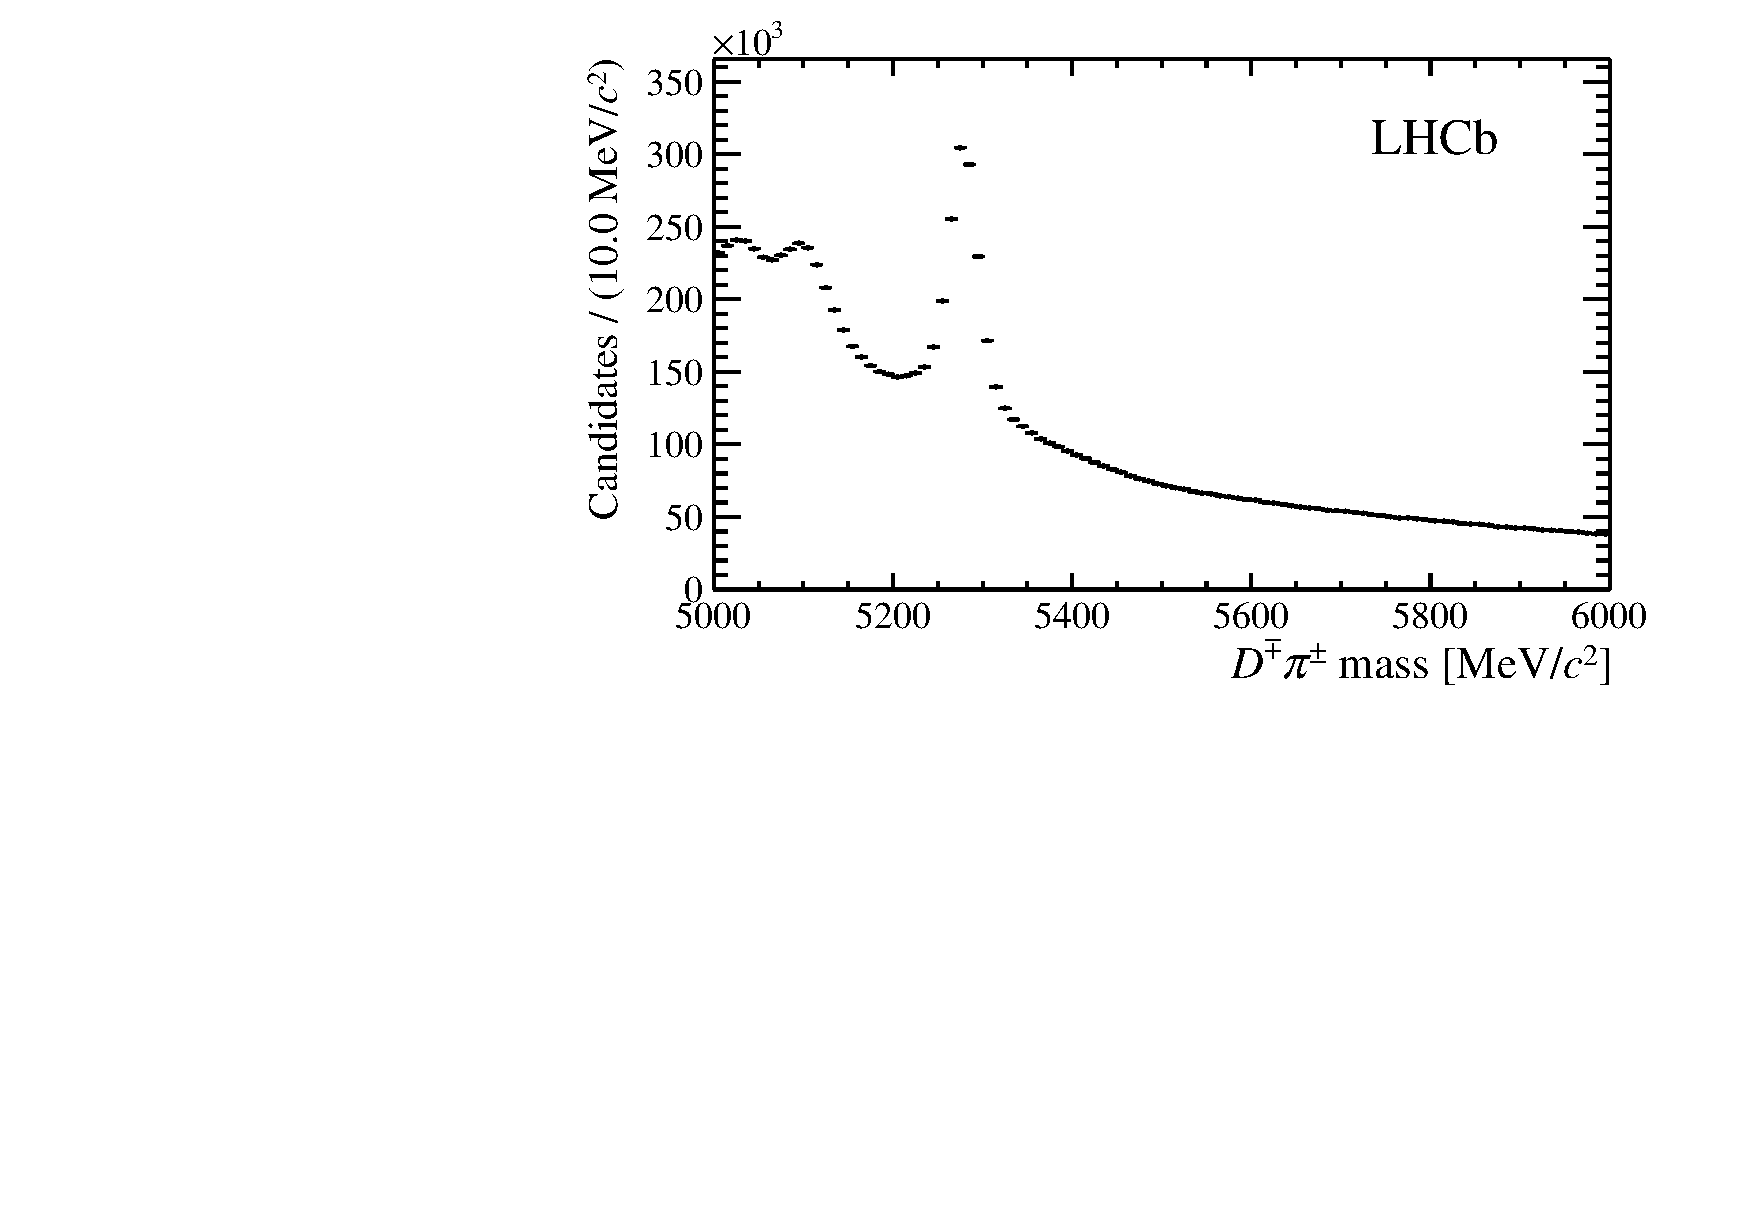
\includegraphics[width=0.45\textwidth]{06selection/figs/Bmass_afterStrippingAndTrigger.pdf}
    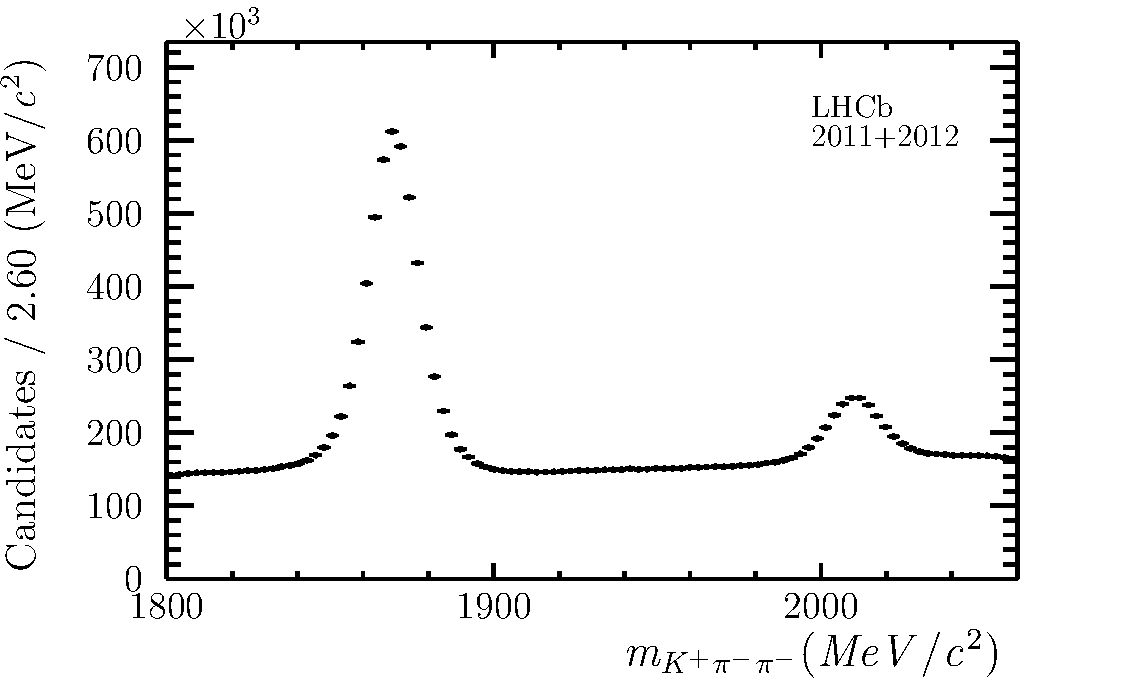
\includegraphics[width=0.45\textwidth]{06selection/figs/Dmass_afterStrippingAndTrigger.pdf}
    \caption{Invariant mass distributions of the $\Dm\pip$ combination using the DTF with a \Dm-mass constrain (right) and of the \Kp\pim\pim combination without any constrain (right).}
    \label{fig:BAndDmassAfterStripping}
\end{figure}

\subsection{Vetoes}
\label{sec:vetoes}

To train and apply a multivariate classifier on data samples, these should at best only consist of signal and combinatorial background.
Therefore backgrounds due to kinematic failures in the reconstruction and wrong associations between a \Bz candidate and a \ac{PV} are vetoed.

\subsubsection*{Mass vetoes}

First, the investigated sources of backgrounds which arise due to failures in the reconstrucion and if necessary the applied vetoes are described.
Such failures can be missed neutral particles or misidentified particles in the reconstruction.

The first type of backgrounds arises from the decay $\Bz\!\to\Dm\mup\neum$. When missing the neutrino and misidentifying the muon as a pion this decay would falsely be reconstructed as the signal decay \BdToDpi.
This is vetoed with a binary requirement on the bachelor particle not to be a muon.
This binary requirement is based on the number and the region of the muon stations where hits are found and the momentum of the track~\cite{Archilli:2013npa}.

The following kinematic backgrounds are all due to misidentification of particles in the finalstate.
Misidentification between protons and pions can lead to backgrounds from $\Lb\!\to\Lcbar\pip$ decays where the \Lcbar decays into a kaon, a pion and an antiproton.
To identify such background candidates a proton-mass hypothesis is applied to both daughter pions of the \Dm-meson.
After combining the three \D daughters again a peak around the \Lc mass becomes visible in the distributionswith shown in \cref{fig:LcVeto}.
The distributions look different, because the pions are originally sorted by transverse momentum \pt.
\begin{figure}[tbp]
    \centering
    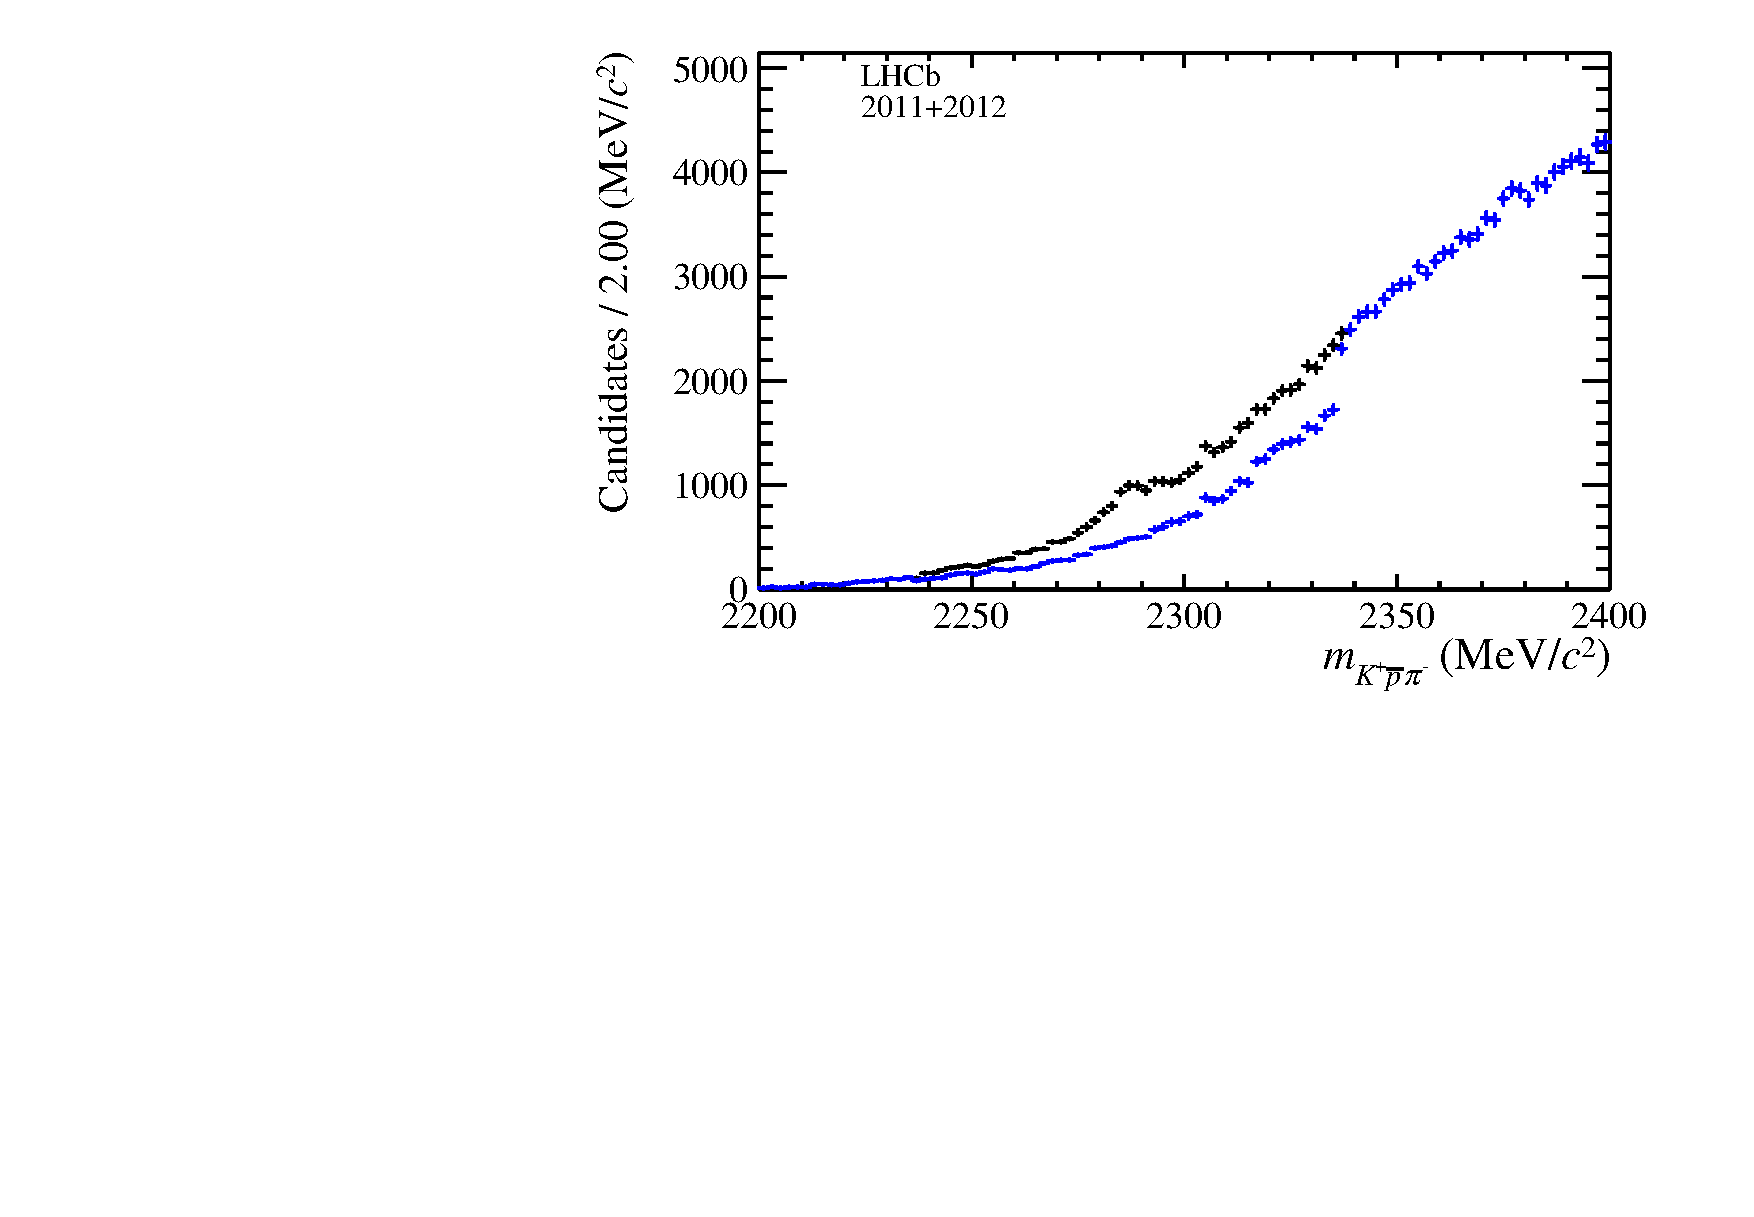
\includegraphics[width=0.45\textwidth]{06selection/figs/LcHypo1.pdf}
    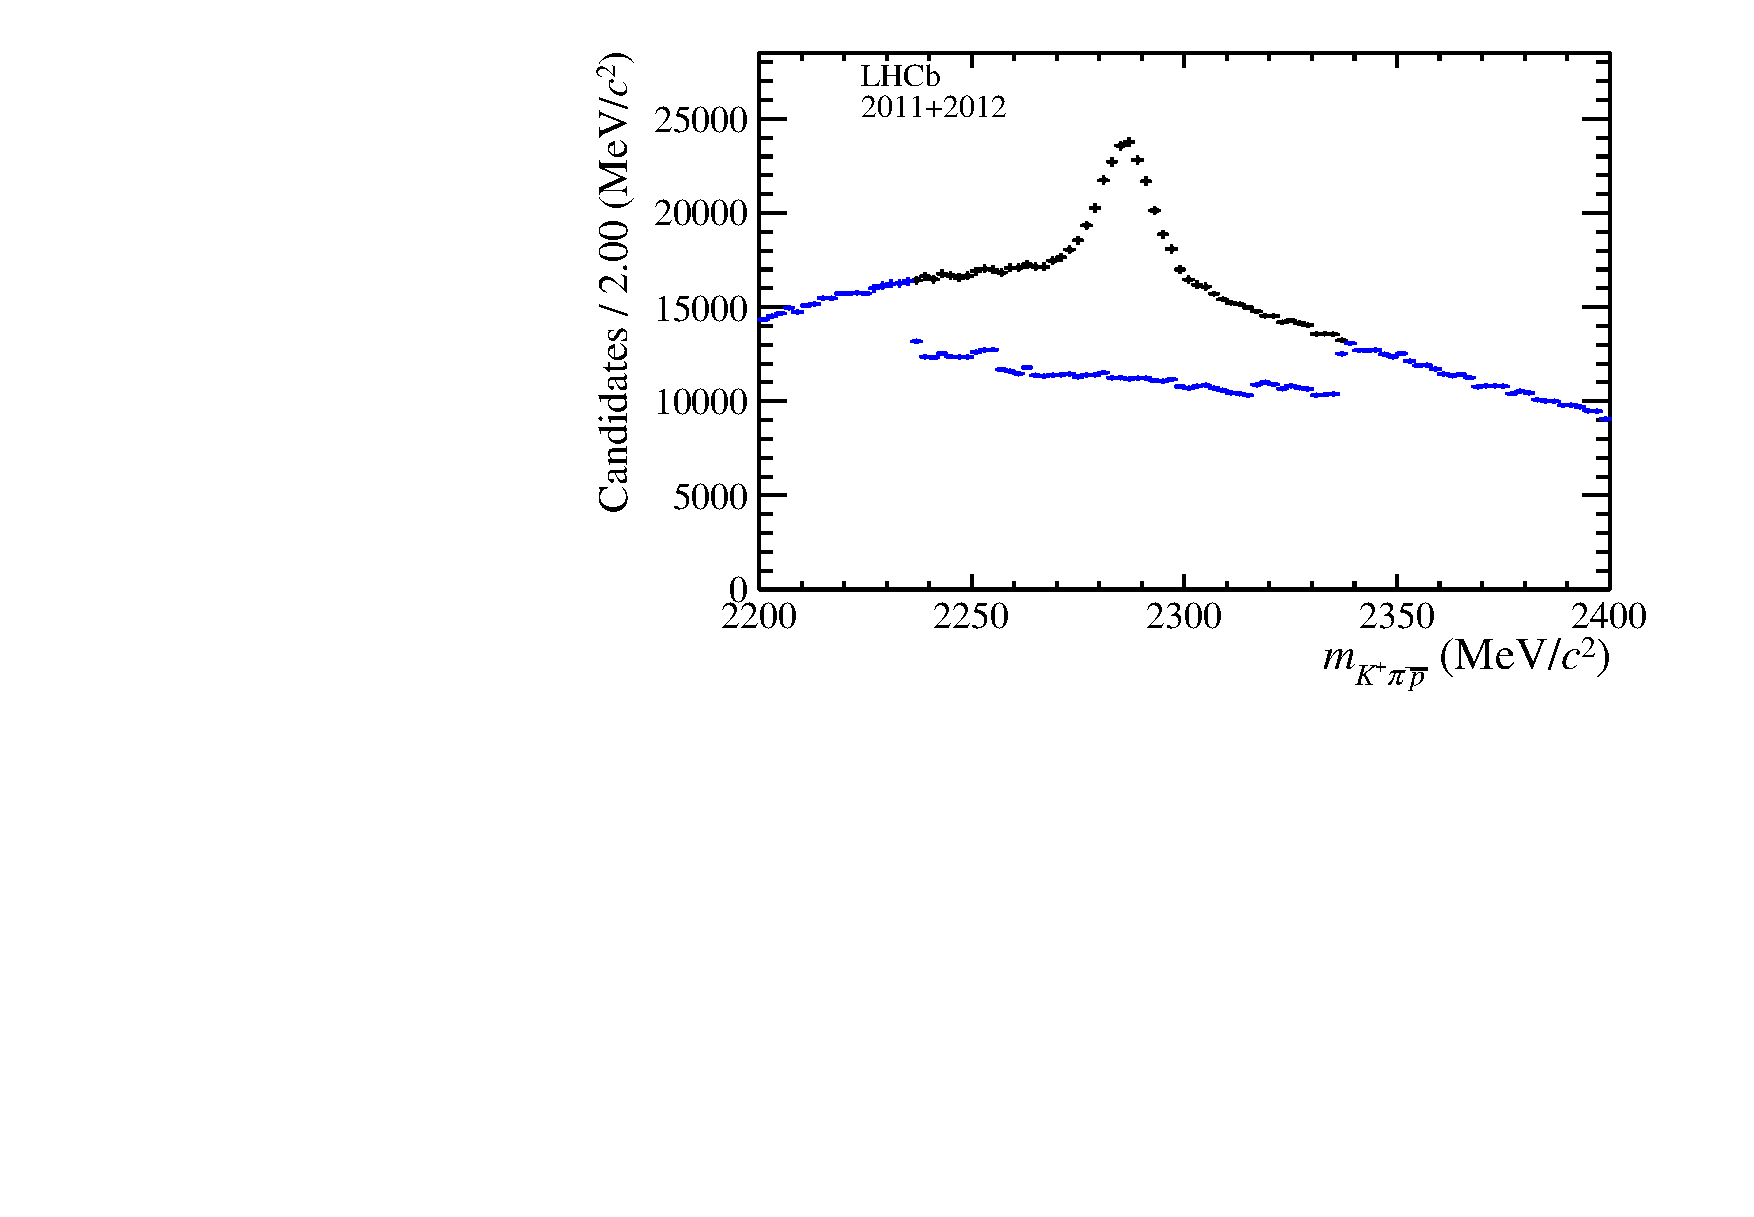
\includegraphics[width=0.45\textwidth]{06selection/figs/LcHypo2.pdf}
    \caption{Invariant mass distributions of the $\kaon\pion\proton$ combinations for both daughter pions of the \Dm-meson.
    The distributions are shown without the veto (black) and with the veto applied (blue).
    In the left plot the proton-mass hypothesis was applied to the pion with lower transverse momentum, right to the pion with higher transverse momentum.}
    \label{fig:LcVeto}
\end{figure}
To remove this background a two-stage veto is applied: In the first stage candidates are rejected if the invariant mass of the three hadrons is inside a \SI[per-mode=symbol]{30}{\MeVcc}  window around the nominal \Lcbar-mass $m_\Lcbar^{\text{PDG}}=\SI[per-mode=symbol]{2286.46}{\MeVcc}$ and the \dllppi is larger than \num{-8.0}.
In the second stage the mass window is enlarged to \SI[per-mode=symbol]{30}{\MeVcc} around the nominal \Lcbar-mass, but the \dllppi is loosened, only requiring $\dllppi>-5.0$.
After the preselection already \SI{99.720\pm0.004}{\percent} of the $\Lb\!\to\Lcbar\pip$ candidates are rejected.
This veto rejects another \SI{76.6\pm0.6}{\percent} at a signal efficiency of \SI{93.48\pm0.06}{\percent}.

In the same way as pions and protons can be misidentified it can happen that a kaon is falsely identified as one of the \Dm daughter pions.
Such misidentification gives rise to a potential background contamination from $\Bs\!\to\Dsm\pip$ candidates.
As before for both pions a kaon mass hypothesis is applied and the three \Dm-daughters are combined.
However,  these distributions do not show a clear mass peak.
Therefore they are compared for different kinematic regions of the invariant $\left[\Kp\pim\pim\right]\pip$ mass: After applying the kaon mass hypothesis, $\Bs\!\to\Dsm\pip$ candidates should end up in the \Bs signal region, whereas no $\Bs\!\to\Dsm\pip$ candidates are expected in the upper-mass sideband $m_{\left[\Kp\pim\pim\right]\pip}>\SI[per-mode=symbol]{5500}{\MeVcc}$.
Therefore the invariant mass distributions of the \kaon\kaon\pion system are compared for candidates from the \Bs signal range \SIrange[per-mode=symbol]{5330}{5400}{\MeVcc} and a background range \SIrange[per-mode=symbol]{5500}{5700}{\MeVcc}.
The visible difference in \cref{fig:DsVeto} stems from the fact that the two distributions arise from different kinematic regions.
\begin{figure}[tbp]
    \centering
    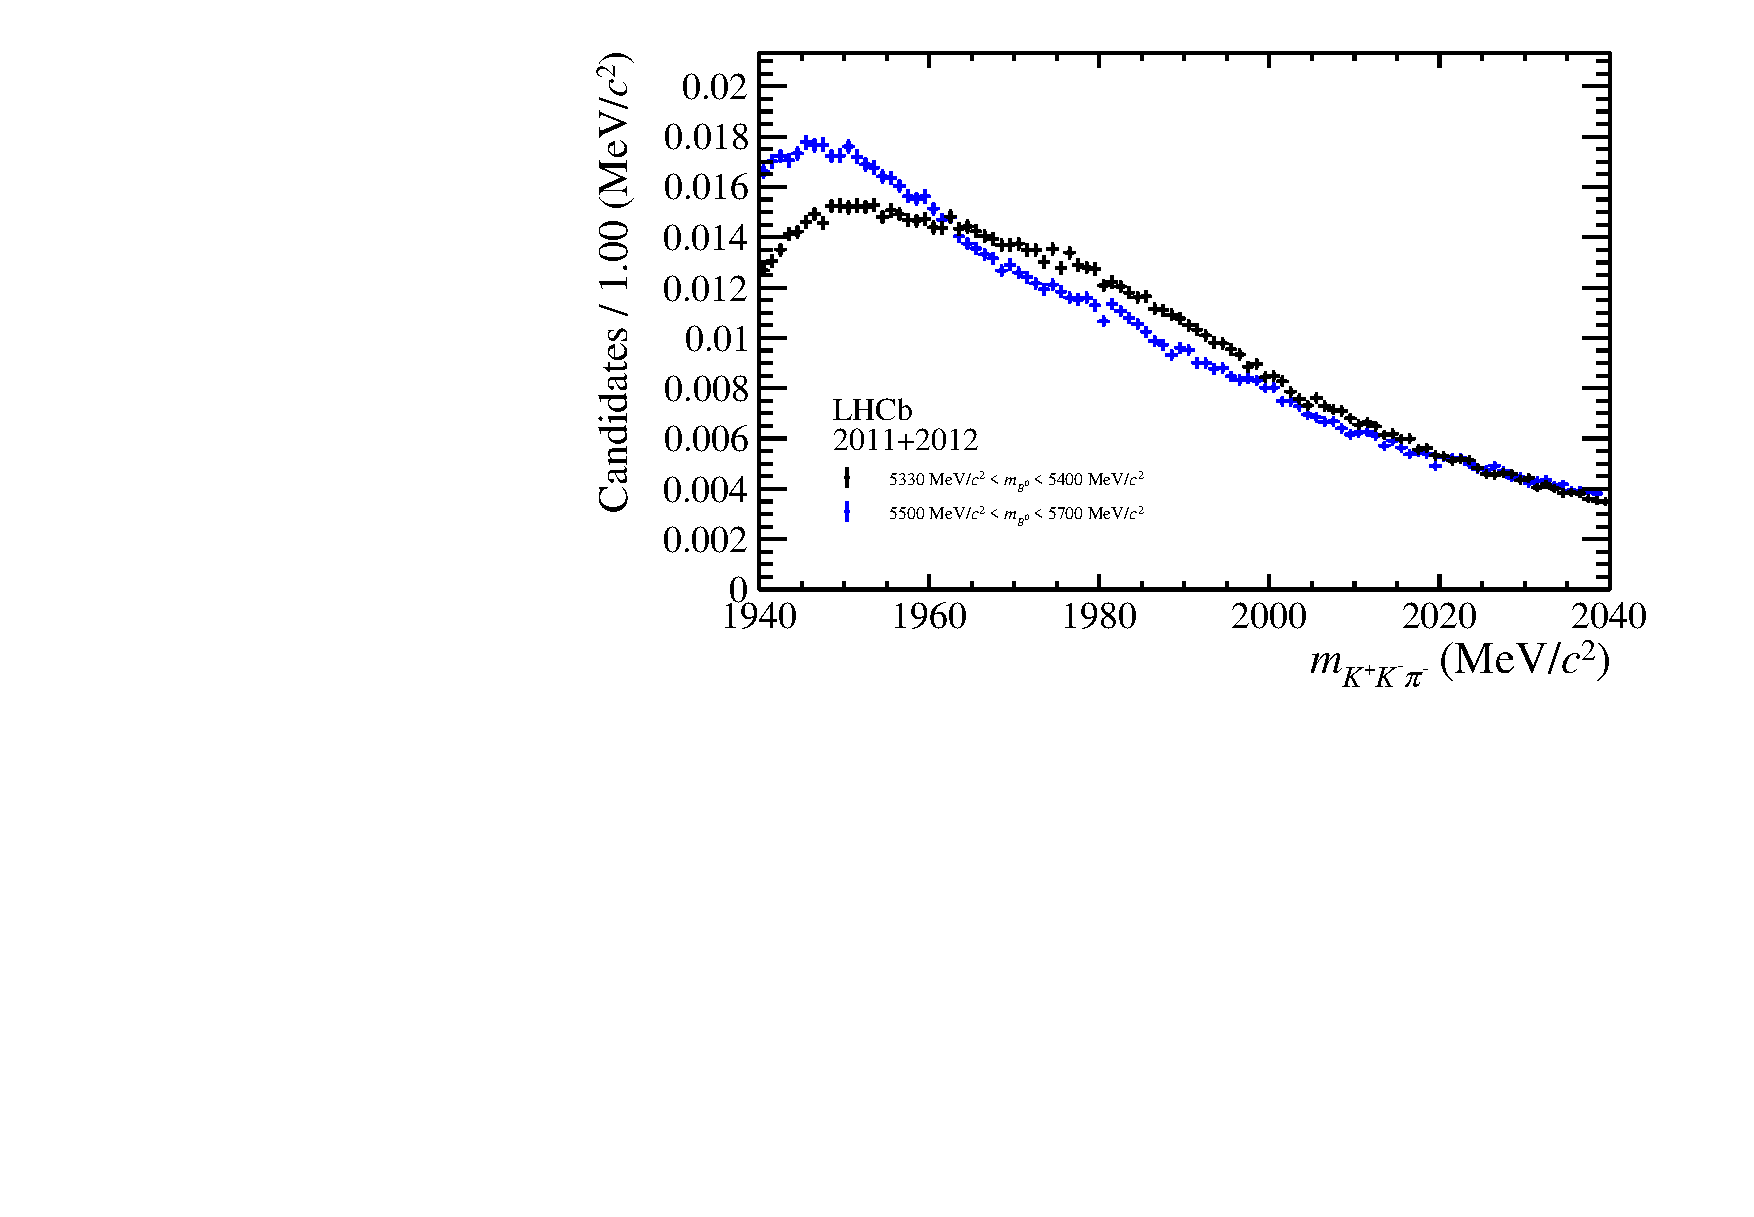
\includegraphics[width=0.45\textwidth]{06selection/figs/DsHypo1.pdf}
    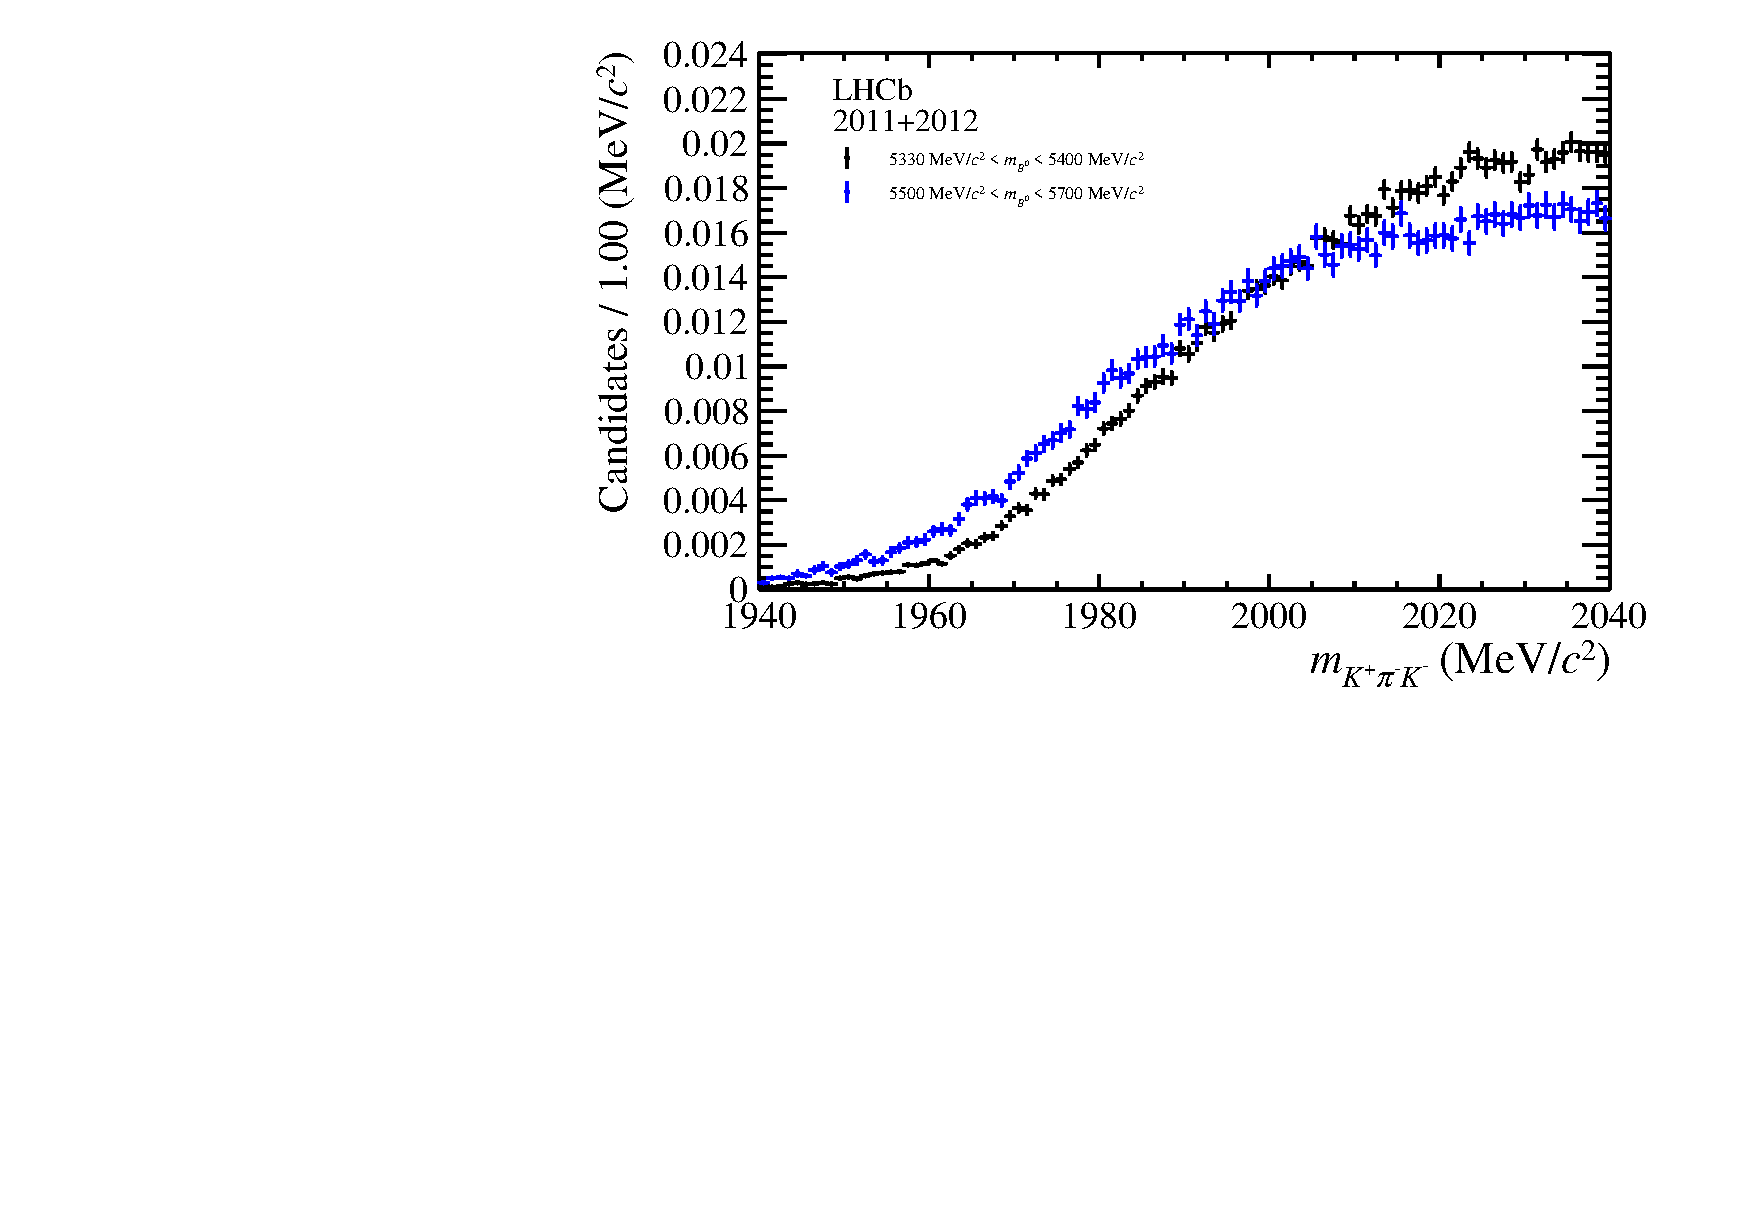
\includegraphics[width=0.45\textwidth]{06selection/figs/DsHypo2.pdf}
    \caption{Invariant mass distributions of the $\kaon\kaon\pion$ combinations for both daughter pions of the \Dm-meson.
    After applying the kaon mass hypothesis the distributions are shown in the \Bs signal region from \SIrange[per-mode=symbol]{5330}{5400}{\MeVcc} (black) and in a background region from \SIrange[per-mode=symbol]{5500}{5700}{\MeVcc} (blue).
    In the left plot the kaon-mass hypothesis was applied to the pion with lower transverse momentum, right to the pion with higher transverse momentum.}
    \label{fig:DsVeto}
\end{figure}
To further ensure that no significant contamination from $\Bs\!\to\Dsm\pip$ candidates is present in the data, resonances like \Kstarz- or $\phi$-mesons, which arise in possible \Dsm decays are studied.
Those resonances would become visible in the \kaon\kaon ($\phi$) and \kaon\pion (\Kstarz) invariant mass distributions.
Figure \ref{fig:phi_Kst_veto} shows exemplary the invariant mass distributions of the \kaon\kaon and \kaon\pion combinations of the pion with larger transverse momentum under the kaon mass hypothesis with the daughter kaon or remaining daughter pion, respectively.
Only candidates within a range from \SIrange[per-mode=symbol]{1940}{2040}{\MeVcc} from \cref{fig:DsVeto} are considered when the distributions are again plotted in the same two kinematic regions as before, \ie in the signal region a peaking structure would be expected in case of a significant contamination with $\Bs\!\to\Dsm\pip$ decays.
As no distribution in \cref{fig:DsVeto} and \cref{fig:phi_Kst_veto} shows such structure, background candidates from $\Bs\!\to\Dsm\pip$ decays are assumed to be negligible.
\begin{figure}[tbp]
    \centering
    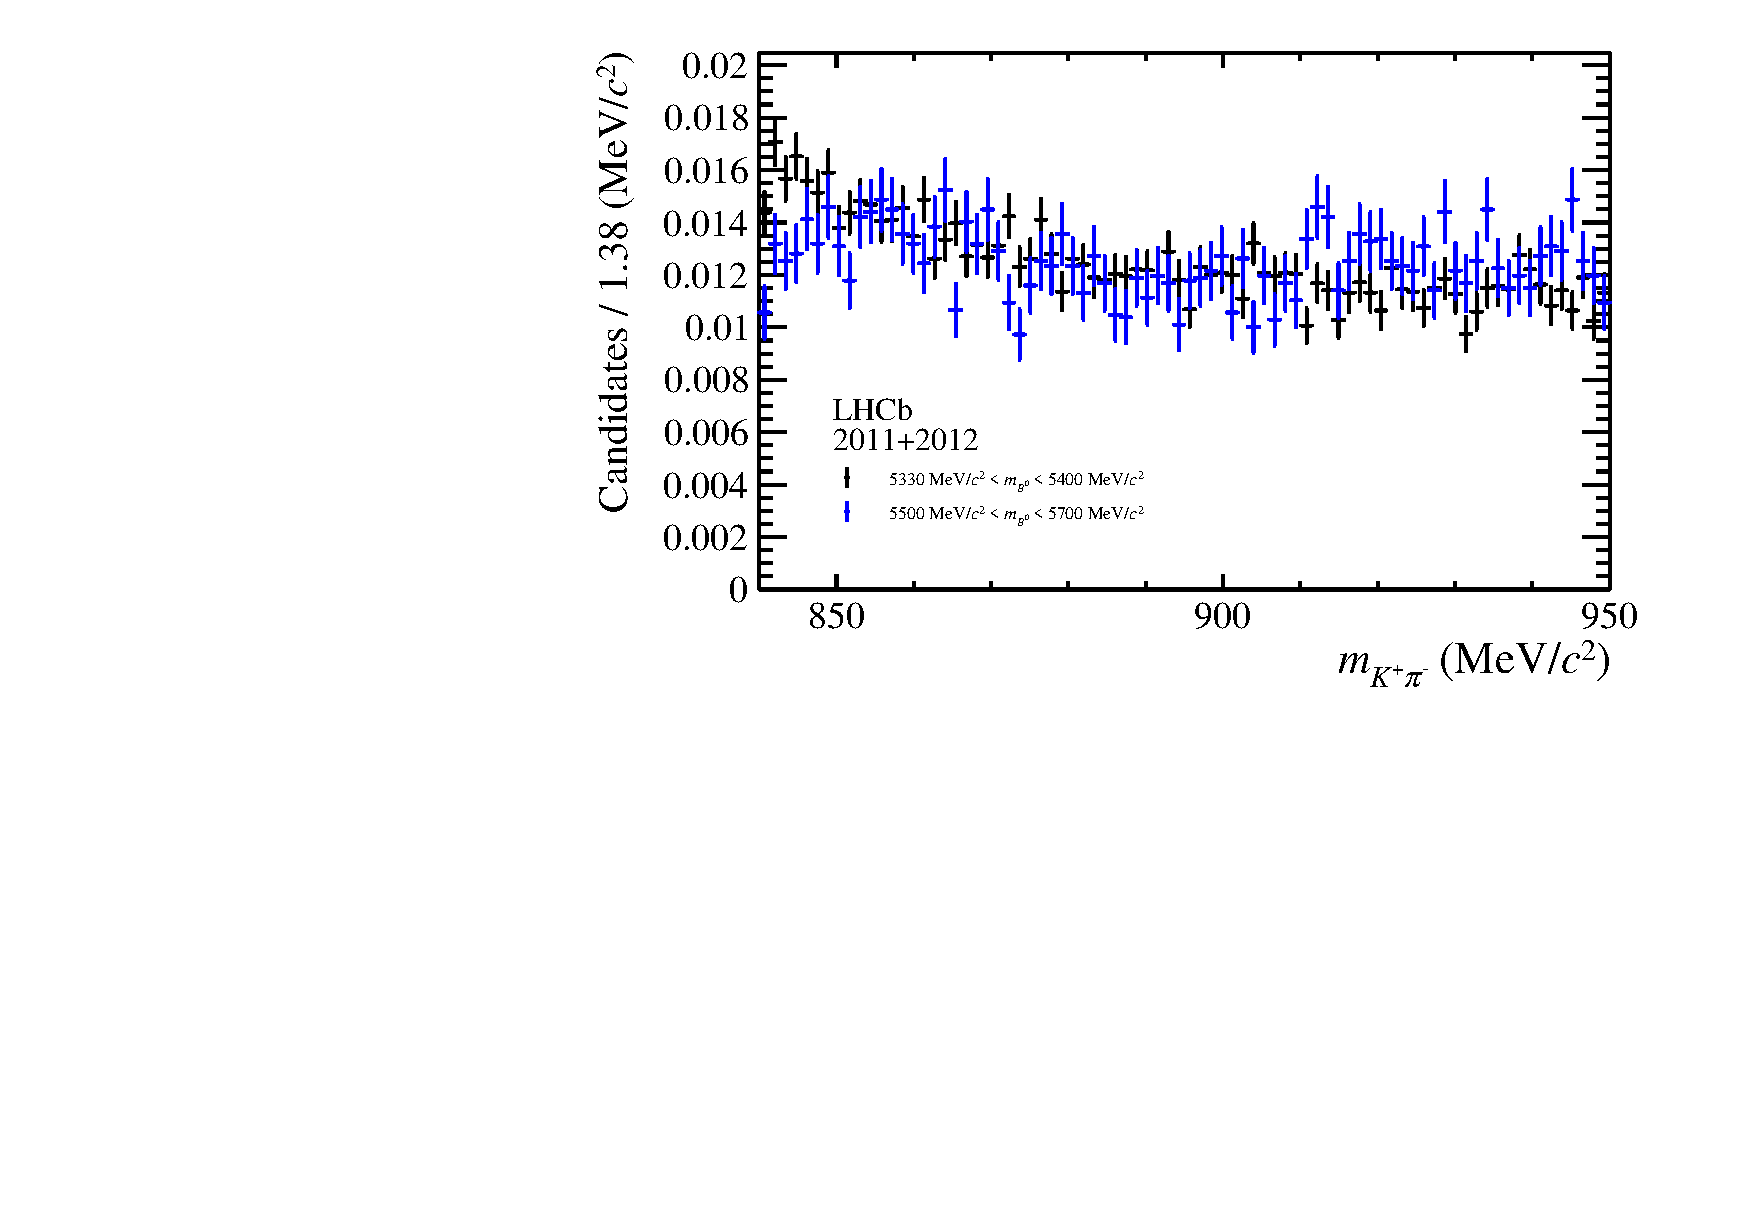
\includegraphics[width=0.45\textwidth]{06selection/figs/KstarHypo2.pdf}
    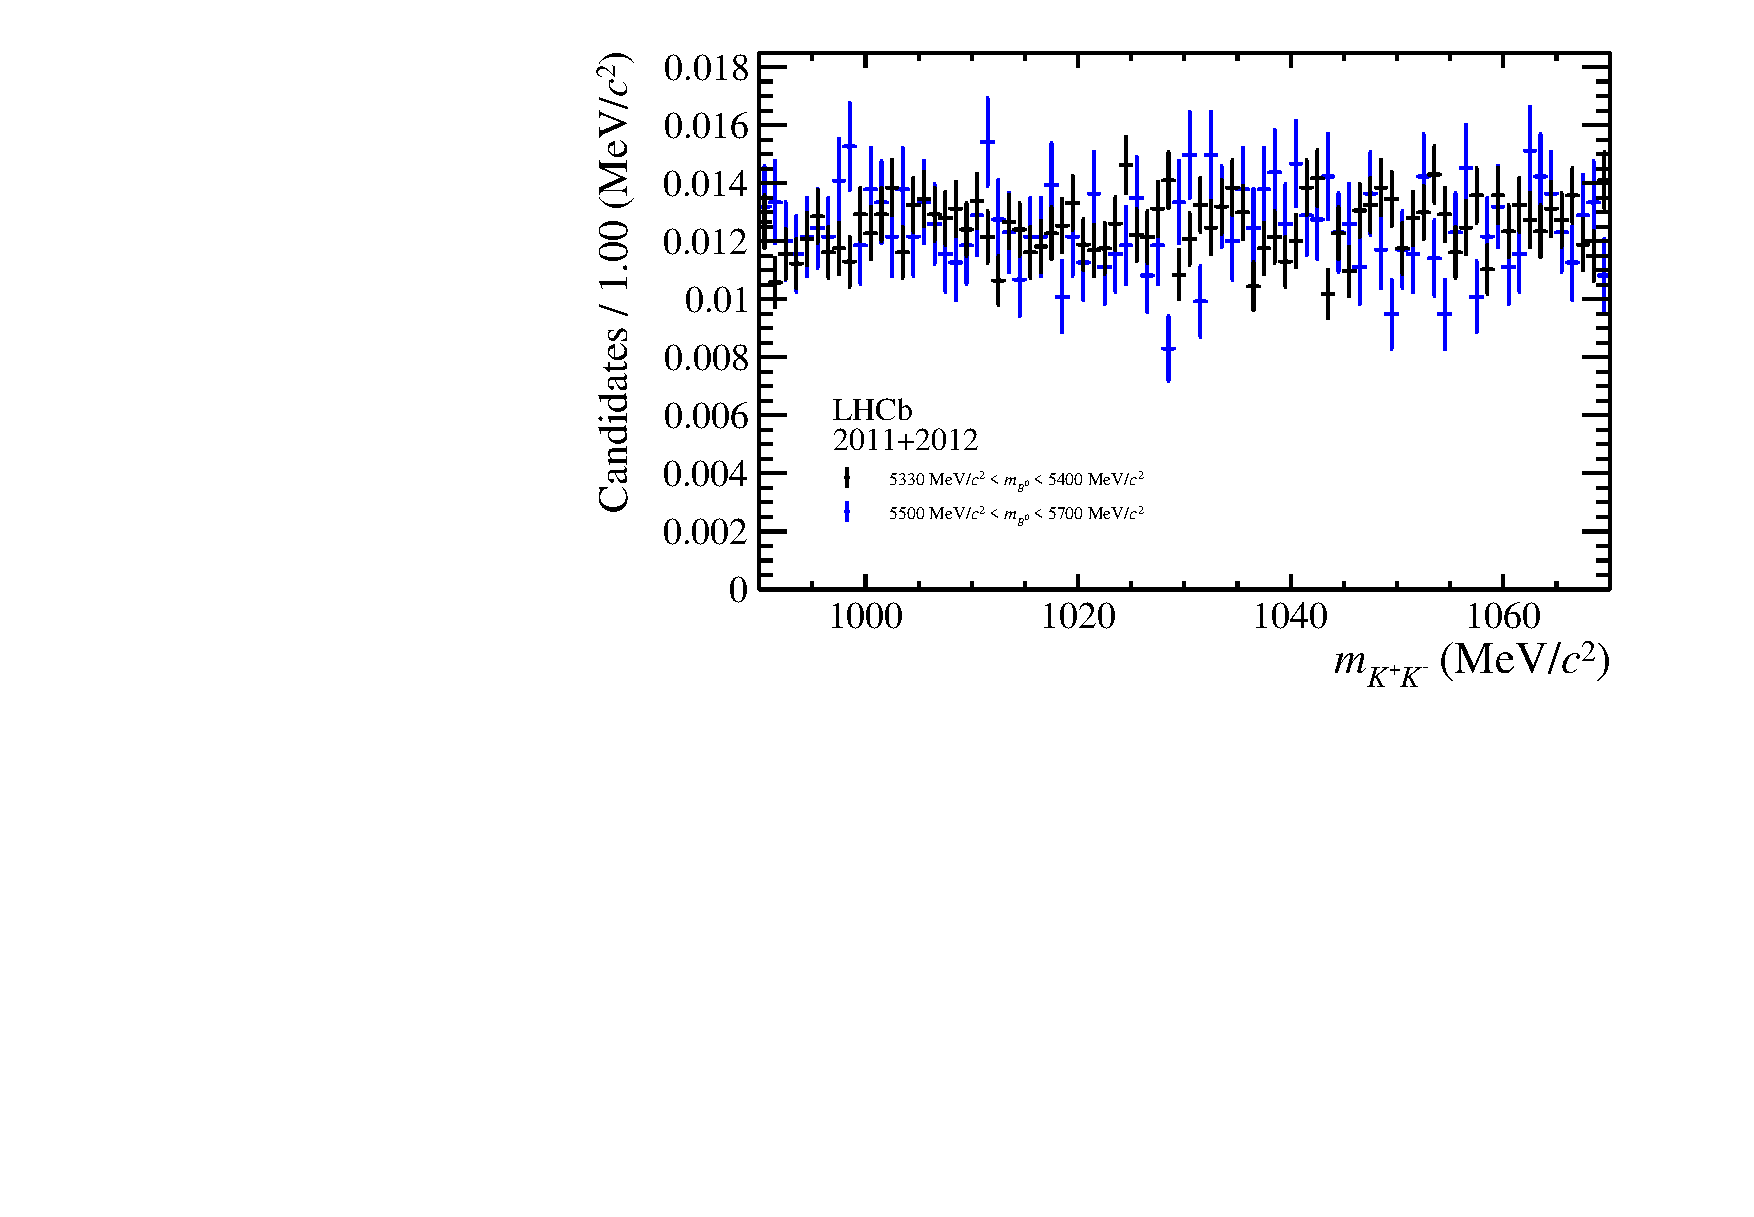
\includegraphics[width=0.45\textwidth]{06selection/figs/PhiHypo2.pdf}
    \caption{Invariant mass distributions of the \kaon\pion (left) and \kaon\kaon (right) combinations for the daughter pion of the \Dm-meson with larger transverse momentum with the daughter kaon or remaining daughter pion, respectively.
    Only candidates with $\SI[per-mode=symbol]{1940}{\MeVcc}<m_{\kaon\kaon\pion}<\SI[per-mode=symbol]{2040}{\MeVcc}$ are considered.
    The invariant mass distributions are shown in the in the \Bs signal region from \SIrange[per-mode=symbol]{5330}{5400}{\MeVcc} (black) and in a background region from \SIrange[per-mode=symbol]{5500}{5700}{\MeVcc} (blue).}
    \label{fig:phi_Kst_veto}
\end{figure}

The last background comes from $\Bz\!\to\DorDbar\kaon\pion$ decays, arising due to a kaon-pion misidentification of the bachelor track or a \Dm-daughter track, followed by a combination the bachelor track with a \Dm-daughter particle.
When doing the four possible combinations of applying the kaon hypothesis to the bachelor particle and the two \Dm-daughter pions all distributions show a flat shape.
Hence, backgrounds from $\Bz\!\to\DorDbar{}^0\kaon\pion$ decays are assumed to be negligible.
In \cref{fig:DzVeto} the combinations of the bachelor track with the \Dm-daughter pion with higher transverse momentum are shown for illustration.
\begin{figure}[tbp]
    \centering
    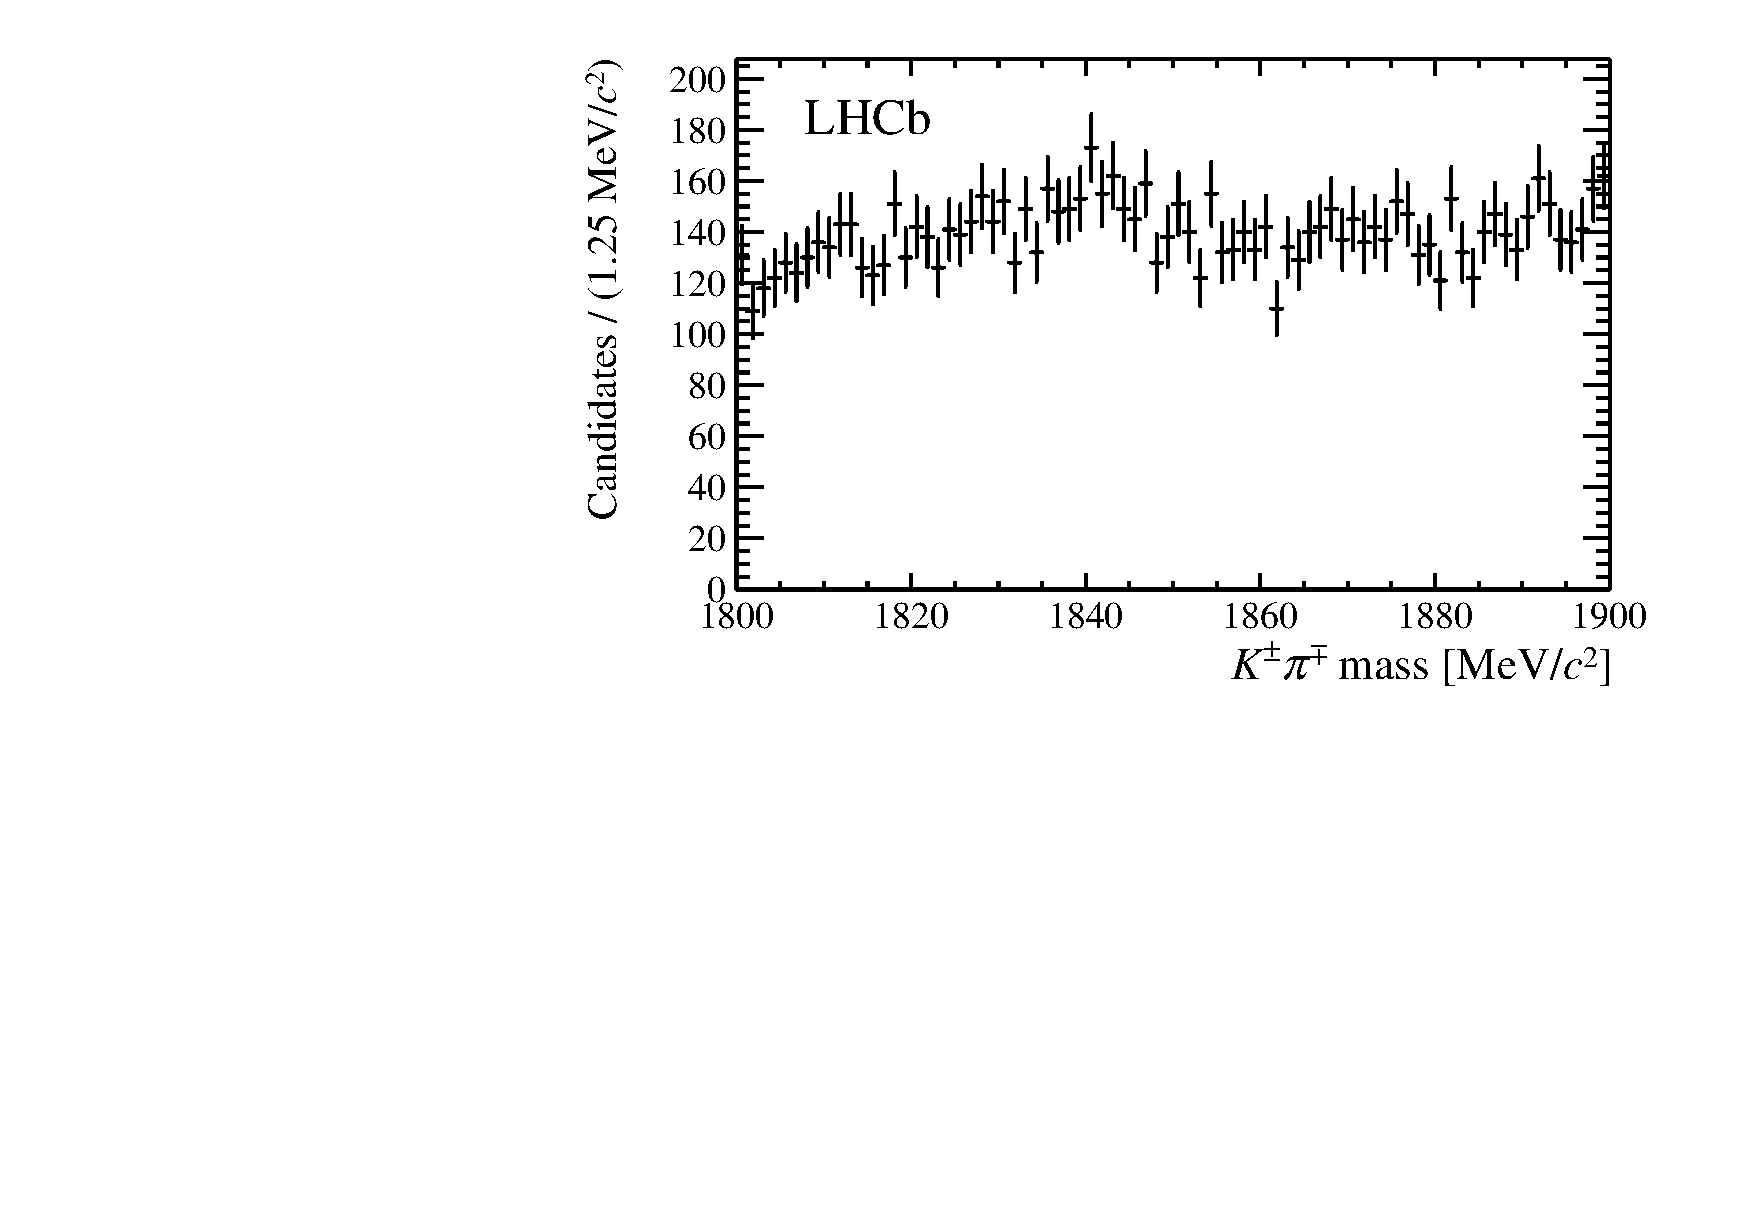
\includegraphics[width=0.45\textwidth]{06selection/figs/D0Hypo3.pdf}
    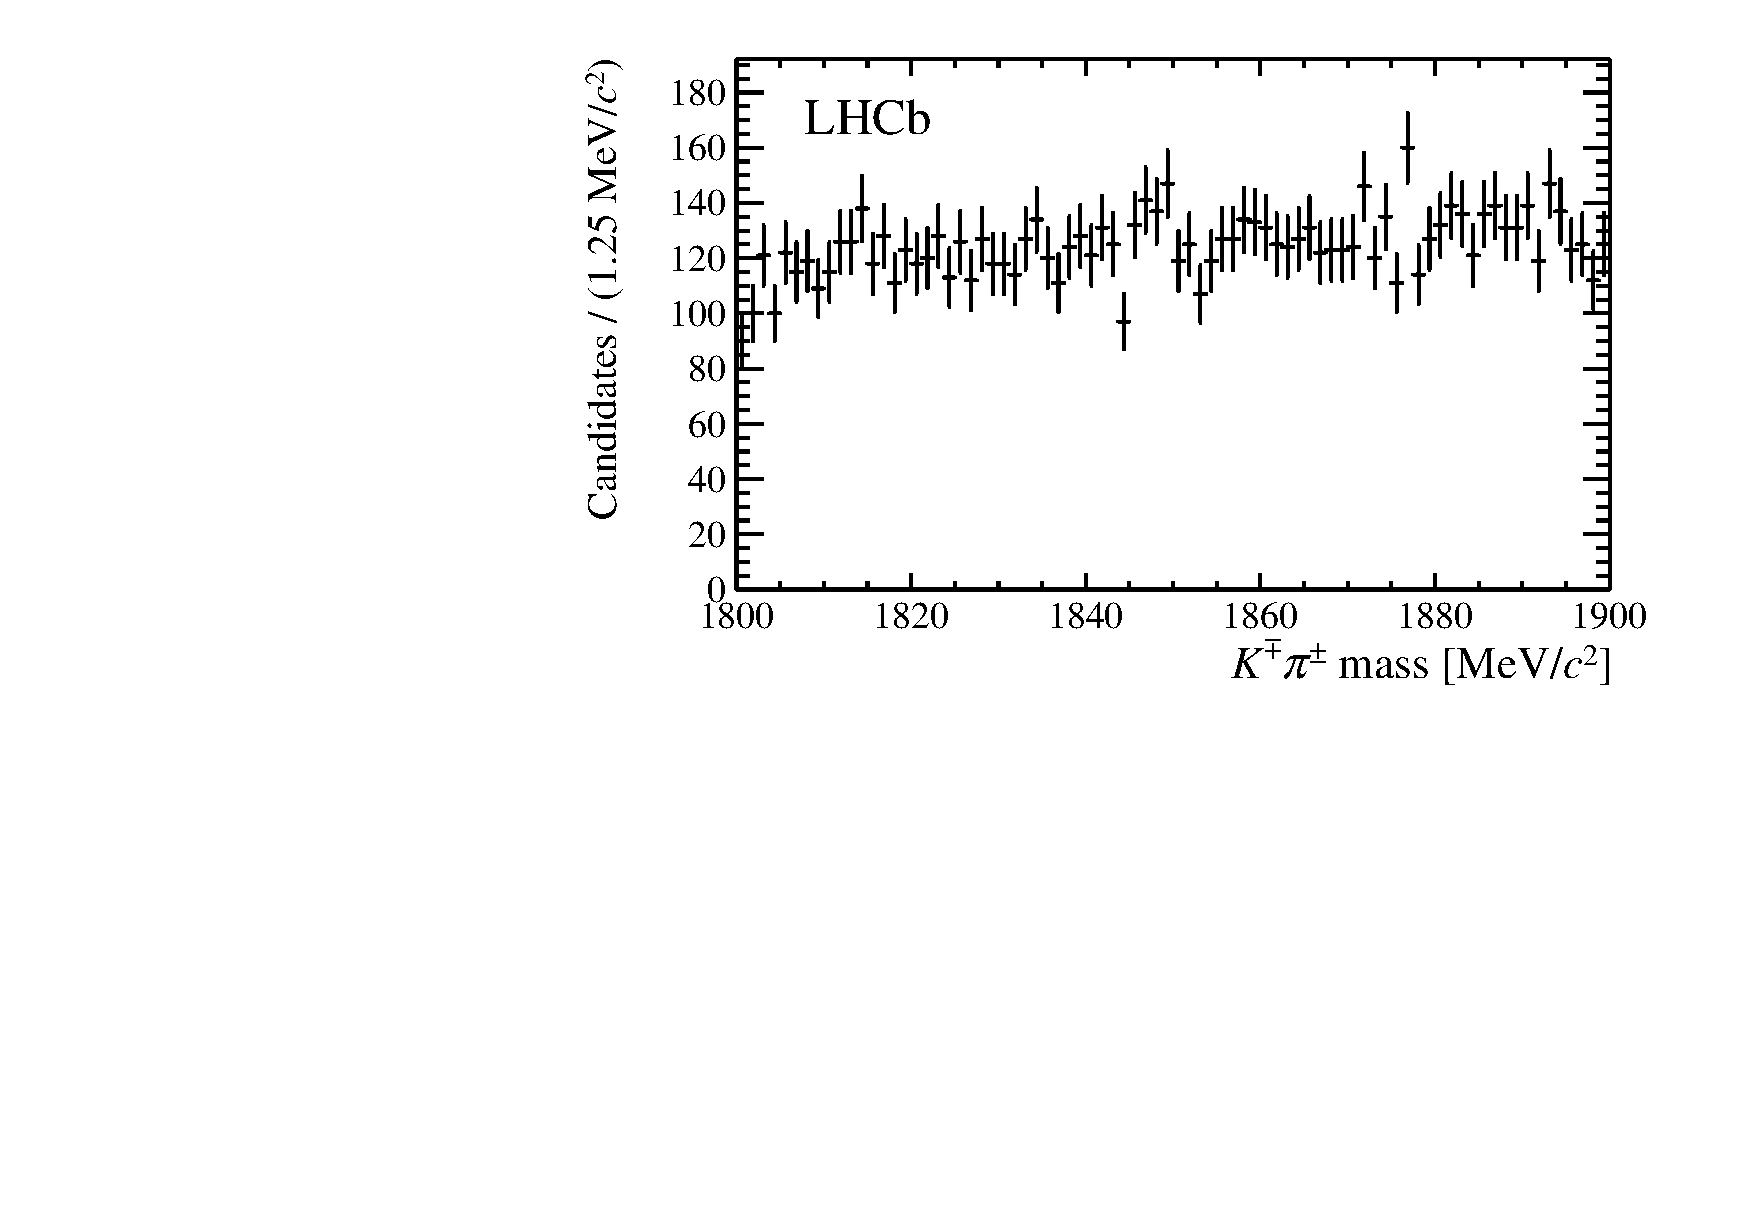
\includegraphics[width=0.45\textwidth]{06selection/figs/D0Hypo4.pdf}
    \caption{Invariant mass distributions for the combinations of the bachelor particle with the \Dm-daughter pion with higher transverse momentum.
    In the left plot the kaon hypothesis is applied to the bachelor pion, in the right plot the kaon hypothesis is applied to the \Dm-daughter pion.}
    \label{fig:DzVeto}
\end{figure}

\subsubsection*{Wrongly associated PVs}

The average number of \proton\proton-collisions per bunch crossing is $\nu=2.5$.
Therefore a considerable amount of events has more than one \ac{PV} and in these events a \Bz candidate can be associated with each of them.
Besides that an event can also contain more than one \Bz candidate; in this case the \Bz candidate is chosen randomly (more details in \cref{sec:MultCands}).
However, in case of multiple \ac{PV}s per event the \Bz candidate can be associated with the wrong PV what leads to a wrong decay time for this candidate.
Usually at \lhcb a decay time dependent selection efficiency is expected, which strongly increases at small decay times up to $\approx\SI{2}{\pico\second}$ and shows a flat or slightly dropping distribution for high decay times.
This efficiency, further denoted as decay time acceptance, is due to the track reconstruction in the \velo and certain trigger requirements.
Yet, due to the wrong \ac{PV} association a large, unexpected tail at high decay times arises.
This can be checked on simulation, where the true decay time is known.
Weighting each (\Bz,\ac{PV})-candidate with an exponential using the true lifetime of the \Bz candidates - \ie (\Bz,\ac{PV})-candidates with high decay times get higher weights - shows an excess of (\Bz,\ac{PV})-candidates at high decay times (see \cref{fig:WrongPVMC}).
\begin{figure}[tbp]
    \centering
    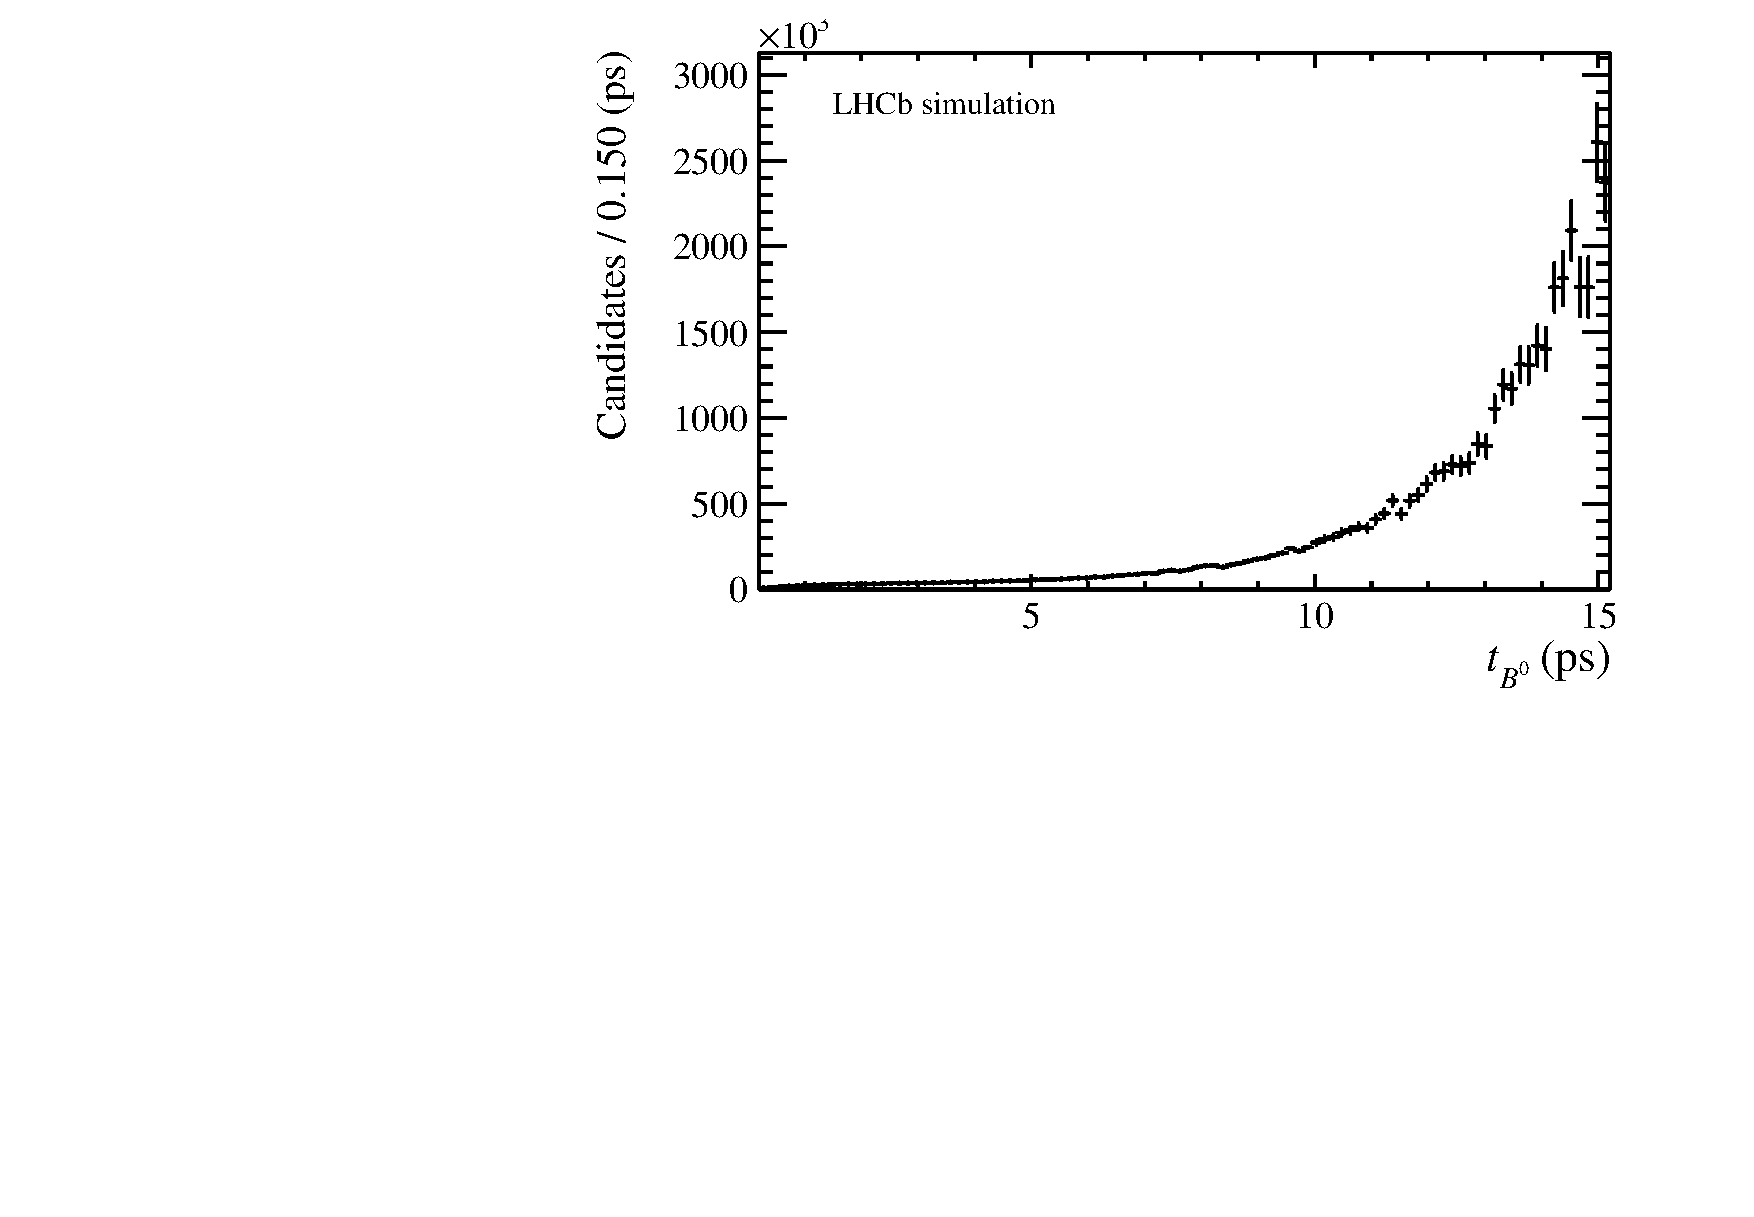
\includegraphics[width=0.45\textwidth]{06selection/figs/WrongPVs-weightedBad.pdf}
    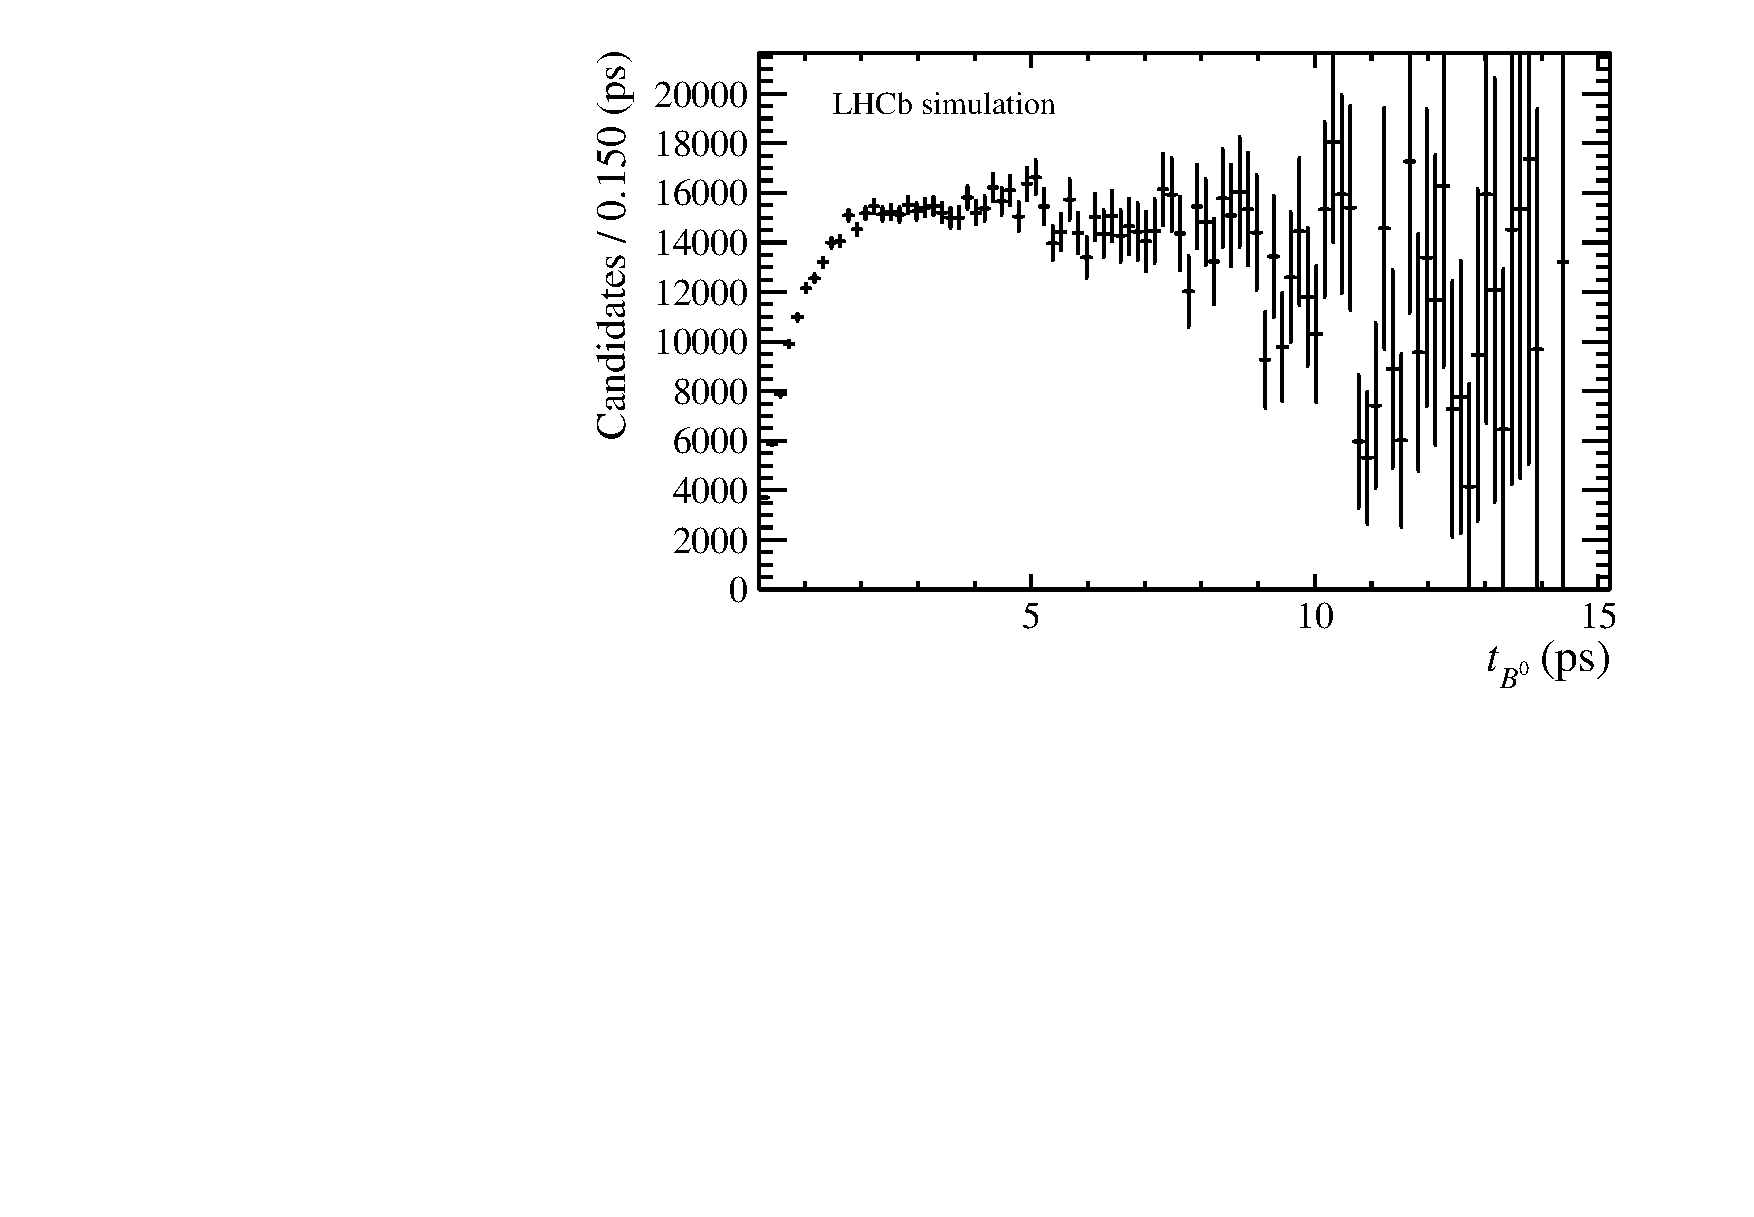
\includegraphics[width=0.45\textwidth]{06selection/figs/WrongPVs-weightedGoodMC.pdf}
    \caption{Left: Decay time distribution of simulated \BdToDpi candidates, wheighted with an exponential using the true lifetime of the \Bz candidates.
    At high decay times an excess of (\Bz,\ac{PV})-candidates can be seen.
    Right: Decay time distribution of simulated \BdToDpi candidates, wheighted with an exponential using the true lifetime of the \Bz candidates after applying a cut on the distance between the true and the reconstructed $z$ position of the \ac{PV}.
    The expected acceptance distribution at \lhcb is visible.}
    \label{fig:WrongPVMC}
\end{figure}
Further on simulation the true $z$-position of the \ac{PV} is known and can be compared with the reconstructed $z$-position.
Requiring that the distance between the true $z$-position of the \ac{PV} and the reconstructed $z$-position does not exceeed five times the uncertainty on the reconstructed $z$-position removes the wrong associated (\Bz,\ac{PV})-candidates from the sample and the expected decay time acceptance becomes visible (\cref{fig:WrongPVMC}).
Though, this approach cannot be applied to data.
Therefore a criterion was developed requiring for each (\Bz,\ac{PV})-candidate the impact parameter $\chi^2_{\text{DTF,PV}}$ with any other \ac{PV} in the event ($\text{MinIP}\chi^2$) to be larger than a certain value.
This means that in case this $\text{MinIP}\chi^2$ is too small, the two corresponding \ac{PV}s cannot be distinguished sufficiently well from each other, and the (\Bz,\ac{PV})-candidate is rejected.
Events which contain just one \ac{PV} are always kept.
The cut is optimised in such a way, that \SI{98}{\percent} of the events in the simulated \BdToDpi sample are retained.
In \cref{fig:WrongPVData} the distribution of the $\text{MinIP}\chi^2$ variable together with the cut point at \num{16.5} and the resulting decay-time-acceptance distribution after applying the \enquote{data} criterion on simulation is shown.
\begin{figure}[tbp]
    \centering
    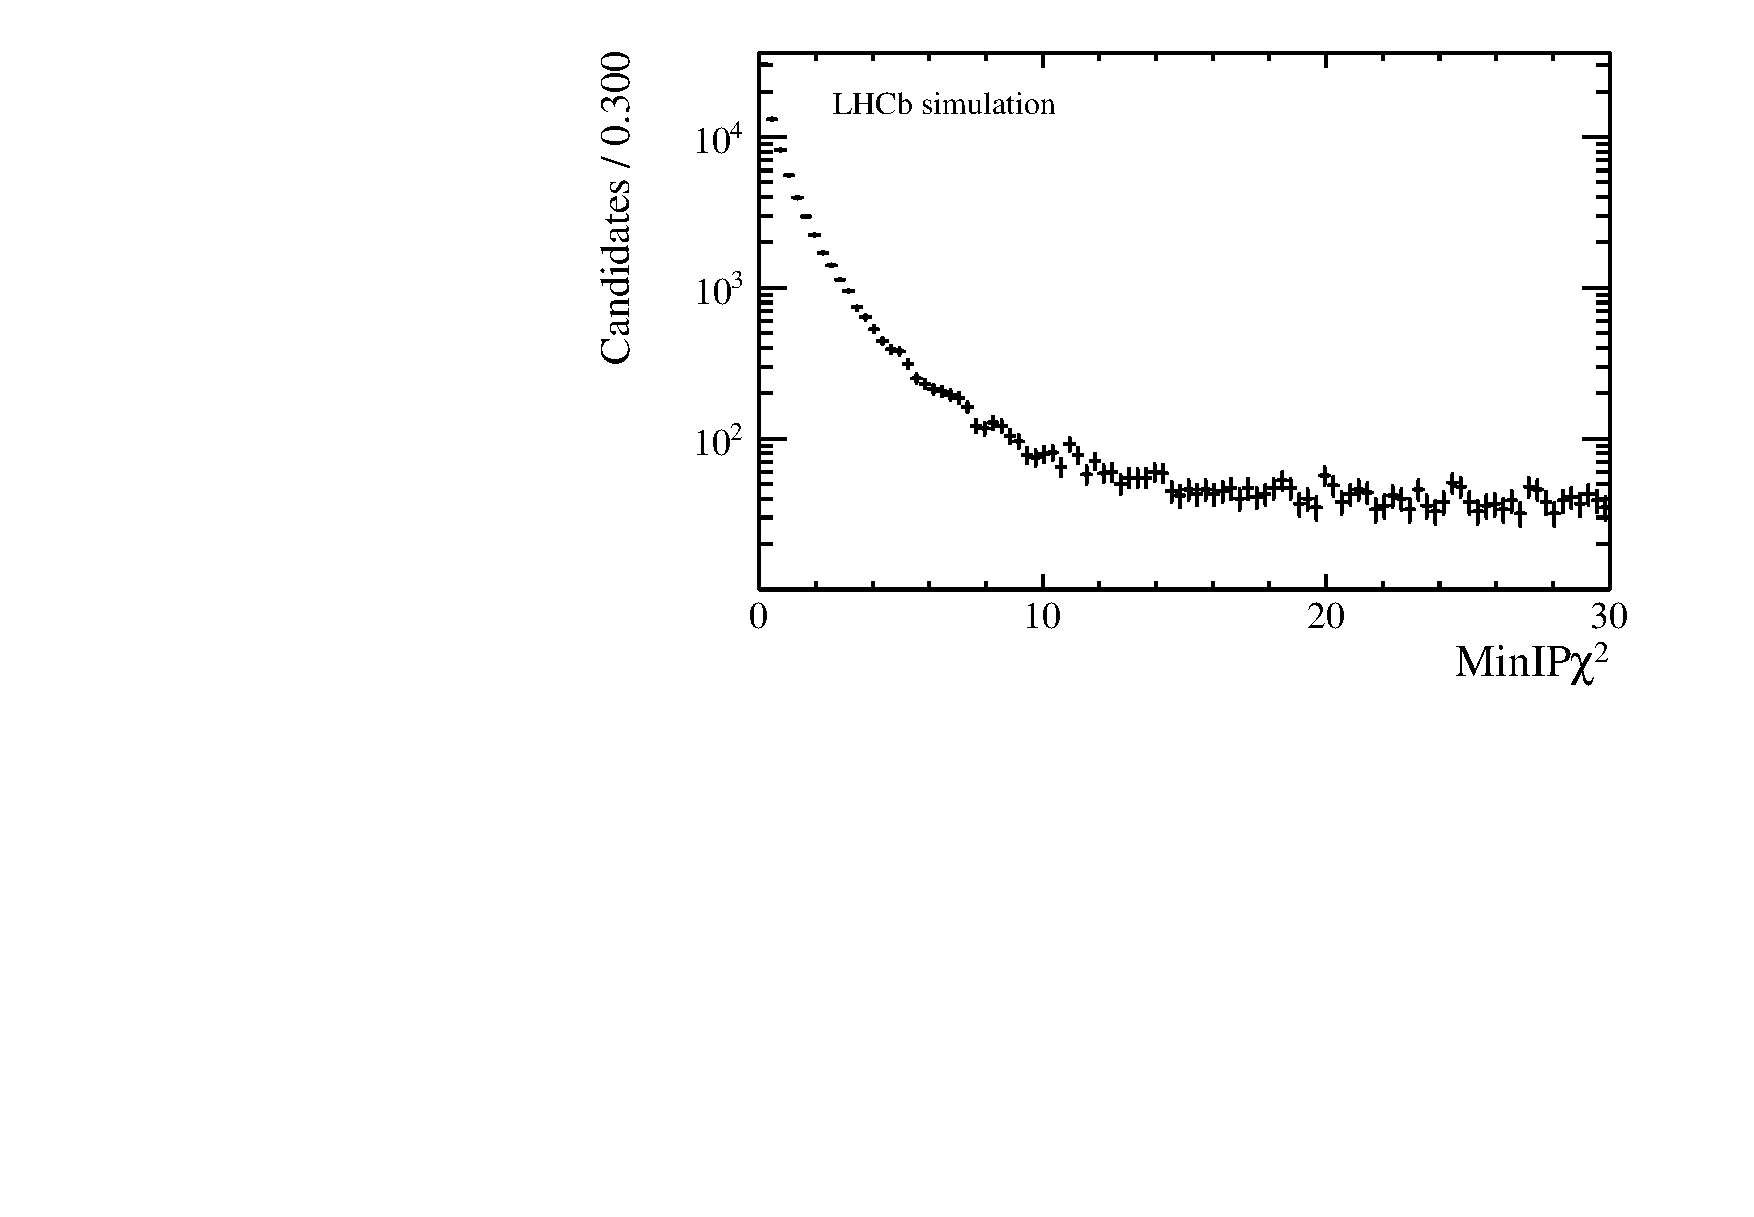
\includegraphics[width=0.45\textwidth]{06selection/figs/MinIPCHI2.pdf}
    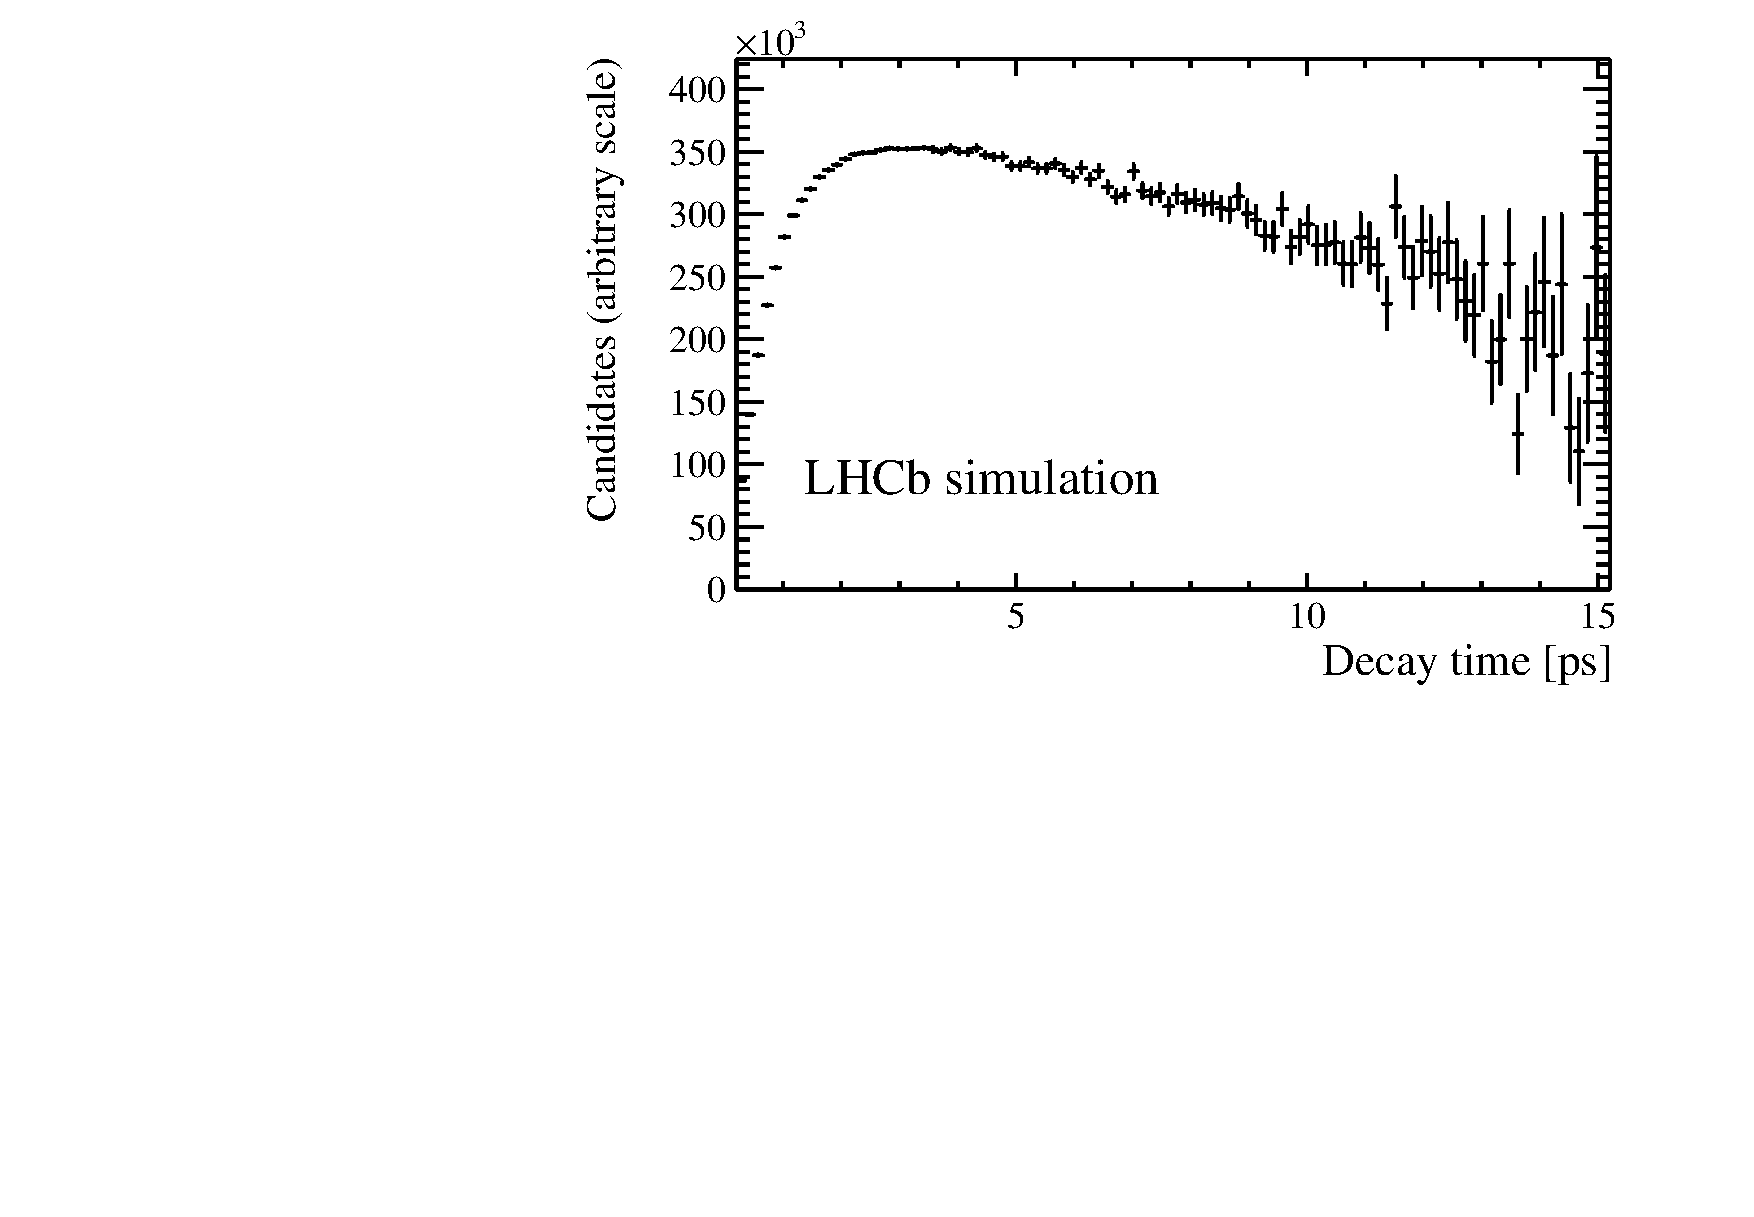
\includegraphics[width=0.45\textwidth]{06selection/figs/WrongPVs-WeightingGoodData.pdf}
    \caption{Left: Distribution of the $\text{MinIP}\chi^2$ variable with the chosen cut point in a narrow range.
    For larger values of $\text{MinIP}\chi^2$ the distribution remains flat.
    Candidates with $\text{MinIP}\chi^2<=16.5$ are rejected.
    Right: Decay time distribution of simulated \BdToDpi candidates, wheighted with an exponential using the true lifetime of the \Bz candidates after applying the cut on $\text{MinIP}\chi^2$.
    The expected acceptance distribution at \lhcb is visible.}
    \label{fig:WrongPVData}
\end{figure}

In contrast the \ac{PV} could also be chosen using some \enquote{best} \ac{PV} criterion, \eg picking the \ac{PV} with the smallest $\text{IP}\chi^2$ w.r.t the \Bz candidate.
Such criterion also removes most of the wrongly associated \ac{PV}s, but it potentially biases the decay time distribution, whereas the strategy described above treats all \ac{PV}s equally and thus the decay time distribution remains unbiased .

\subsection{Development of a MVA classifier}
\label{sec:MVADev}

Combinatoric background is suppressed using a \ac{MVA}, more precisely a \ac{BDT} is used.
A \ac{BDT} is a machine learning algorithm for classification.
As all machine learning algorithms it needs to learn, which classes of events should be be separated.
Therefore it needs training samples, consisting only of events of the respective classes.
In this case \BdToDpi candidates should be separated from combinatorial background candidates and therefore it needs to be provided with proxies for these classes of candidates.
As proxy for the \BdToDpi candidates, simulation is used based on the conditions of the \num{2012} data taking.
The upper-mass sideband of the \num{2012} data with $m_{\left[\Km\pip\pip\right]\pim}>\SI[per-mode=symbol]{5500}{\MeVcc}$ mimics the background.
Further both proxy samples are divided into a training and a test sample of same size.
When training the \ac{BDT}, the training part is used to actually classifiy the candidates, while the \ac{BDT} can be applied on the independent test sample, to check whether the performance is the same on both samples.
If the performance is different between the samples, the \ac{BDT} shows so-called overtraining, \ie the classifier is optimised on statistical fluctuations of the training samples and cannot be applied to other independent samples without a loss in performance.
Another powerful test to check for overtraining is to compare the output distribution of the \ac{BDT} between the training and test sample - again, a difference would indicate that the \ac{BDT} is overtrained.
As also in the analysis the \ac{BDT} should learn to separate signal candidates from combinatoric background after applying the vetoes and removing backgrounds like $\Lb\!\to\Lcbar\pip$, all previous selection steps are applied to the signal- and background-proxy samples.

The \ac{BDT} uses in total \num{16} input variables which are listed in \cref{tab:BDTInput}.
To reduce the number of input variables, for pairs of variables which had a correlation of \SI{97}{\percent} or larger the variable with the smaller separation power was removed.
The final variables cover mostly various $\text{IP}\chi^2$ variables, flight distances, momenta and flight directions.
Furthermore the $\chi^2$ of the DTF with a constraint on the \ac{PV} is added, as it shows a good separation power between \BdToDpi signal candidates and combinatoric background candidates.
\begin{table}[tbp]
	\centering
	\caption{List of input variables used in the training of the BDT}
	\begin{tabular}{cc}
		\toprule
		\multirow{2}{*}{\Bz candidate}	& $\cos$ of $\sphericalangle\left[\left|\text{PV},\text{SV}\right|,\vec{p}\!(\Bz)\right]$ \\
										& \ac{SV} $\chi^2$\\
		\midrule
		\multirow{7}{*}{\Dm candidate}	& $\text{IP}\chi^2$ w.r.t. the \ac{SV}\\
										& $\text{IP}\chi^2$ w.r.t. the associated PV\\
										& radial flight distance\\
										& flight distance $\chi^2$ w.r.t. the \ac{SV}\\
										& \Dm-vertex $\nicefrac{\chi^2}{\text{ndof}}$\\
										& transverse momentum \pt \\
										& $\cos$ of $\sphericalangle\left[\left|\text{SV},\Dm\text{-Vtx}\right|,\vec{p}\!(\D)\right]$ \\
		\midrule
		\multirow{3}{*}{bachelor \pion}	& $\text{IP}\chi^2$ w.r.t. the associated PV\\
										& transverse momentum \pt\\
										& track $\nicefrac{\chi^2}{\text{ndof}}$\\
		\midrule
		\Dm daughters					& $\text{IP}\chi^2$ of the associated \ac{PV}\\
		\midrule
		DTF 							& $\chi^2$ of the DTF with \ac{PV} constrain \\
		\bottomrule
	\end{tabular}
	\label{tab:BDTInput}
\end{table}
For the \ac{BDT} the implementation from TMVA~\cite{Hocker:2007ht} is used.
The \ac{BDT} consists of \num{1700} decision trees with a maximum depth of four.
The variables are scanned at \num{20} points to find the optimal cut value and each node has to contain at least \SI{2.5}{\percent} of the training candidates.
For the boosting the AdaBoost algorithm~\cite{AdaBoost} was chosen with a boost factor $\beta=0.5$.
The approach to find this configurations was iteratively, \ie the complexity of the \ac{BDT} was increased as long as no overtraining was visible.
The final overtraining check is shown in \cref{fig:BDTOVertraining}.
\begin{figure}[tbp]
    \centering
    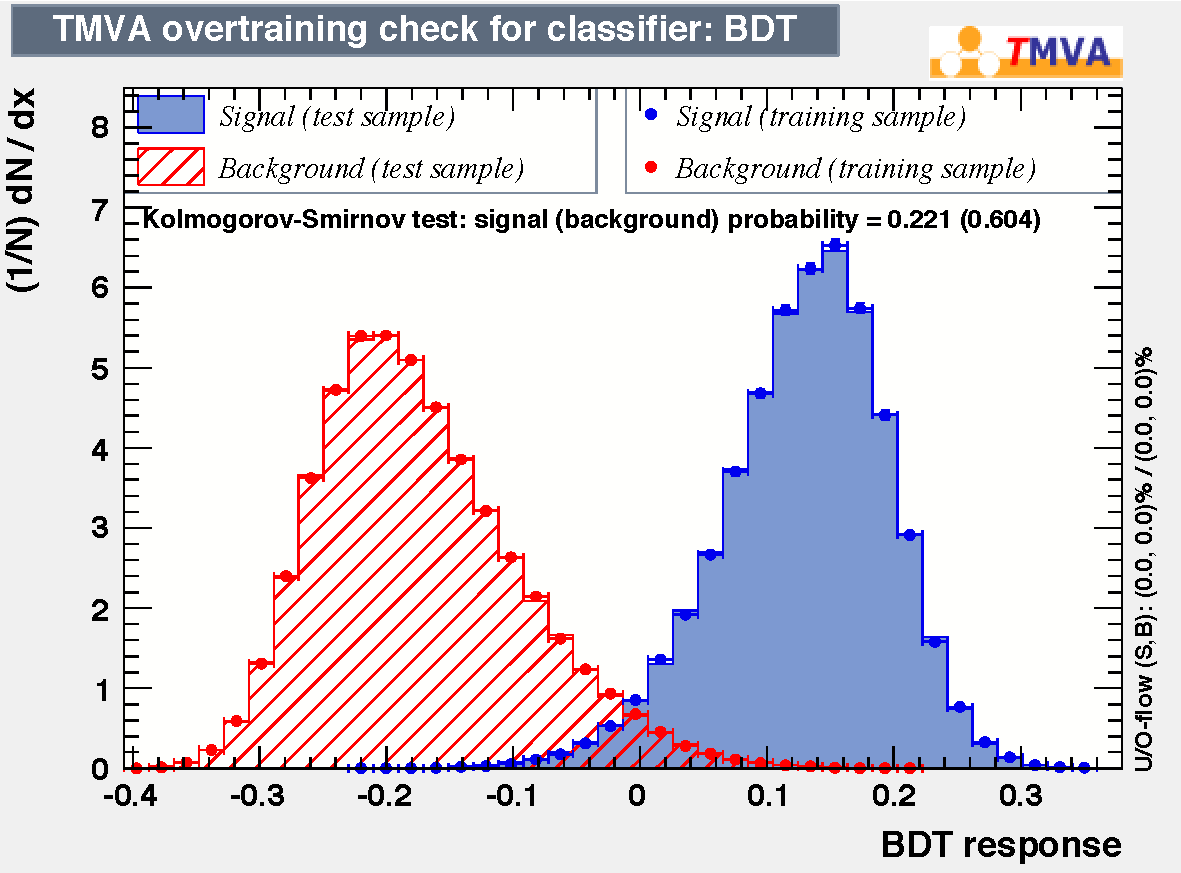
\includegraphics[width=0.7\textwidth]{06selection/figs/overtrain_BDT.pdf}
    \caption{Comparison of \ac{BDT} responses on the training and test sample.}
    \label{fig:BDTOVertraining}
\end{figure}
The agreement between the \ac{BDT} output distributions on the training and test samples is also checked with a Kolmogorov-Smirnov test which gives \num{0.221} and \num{0.604} for the signal and background samples and thus indicates a good agreement.

\subsection{BDT selection optimisation}
\label{sec:BDTOpt}

To optimise the cut on the \ac{BDT} response the uncertainties on the \CP parameters \Sf and \Sfbar are used.
For the optimisation all preselection cuts, the vetoes for background from semileptonic decays and $\Lb\!\to\Lcbar\pip$ decays and the veto for wrongly associated \ac{PV}s are applied to the full dataset of both Run I.
To determine the uncertainty of \Sf and \Sfbar depending on the \ac{BDT} response the following strategy is adopted:
The \ac{BDT} output is scanned with a step size of \num{0.01} within a narrow range from \numrange{-0.15}{0.1} and with a step size of \num{0.05} in the outer regions.
For each cut on the \ac{BDT} response a fit to the invariant \Bz mass in the range \SIrange[per-mode=symbol]{5200}{5500}{\MeVcc} using the \emph{pion}-sample is performed.
This fit is used to determine \emph{sWeights}~\cite{Pivk:2004ty} and to obtain the mass shape which corresponds to the respective cut on the \ac{BDT} output.
Applying the \emph{sWeights} to other observables as the decay time, makes these distributions appear as signal-only~\cite{2009arXiv0905.0724X}.
Therefore, using \emph{sWeights} the tagging efficiencies, the shapes of the mistag distributions of the OS and SS tagging algorithms (more details on the flavour tagging can be found in \cref{ch:flavourtagging}) and the shape of the decay-time acceptance are obtained for the \enquote{signal} distributions.
The shape of the decay-time acceptance is obtained by fitting the decay-time distribution with a fixed lifetime and only floating the parameters of a cubic b-spline-model~\cite{splines}.
For each cut point then a single pseudoexperiment is performed: The invariant mass distribution is generated using the obtained signal and background yields and shapes from the mass fit, for the mistag and decay time distribution signal and background are both generated using the signal shapes.
The generated values for the \CP parameters are taken from simulation.
This pesudoexperiment sample is then fitted back: After determining \emph{sWeights} from a fit to the invariant \Bz mass distribution, a \CP fit to the decay time distribution is performed, where the flavour tagging calibration is assumed to be perfect.
In \cref{fig:BDTopt} the uncertainties on \Sf and \Sfbar are shown as a function of the \ac{BDT} response.
The final cut point is chosen at the right end of the plateau at \num{0.0}, to have as few background as possible while achieving the best possible sensitivity.
\begin{figure}[tbp]
    \centering
    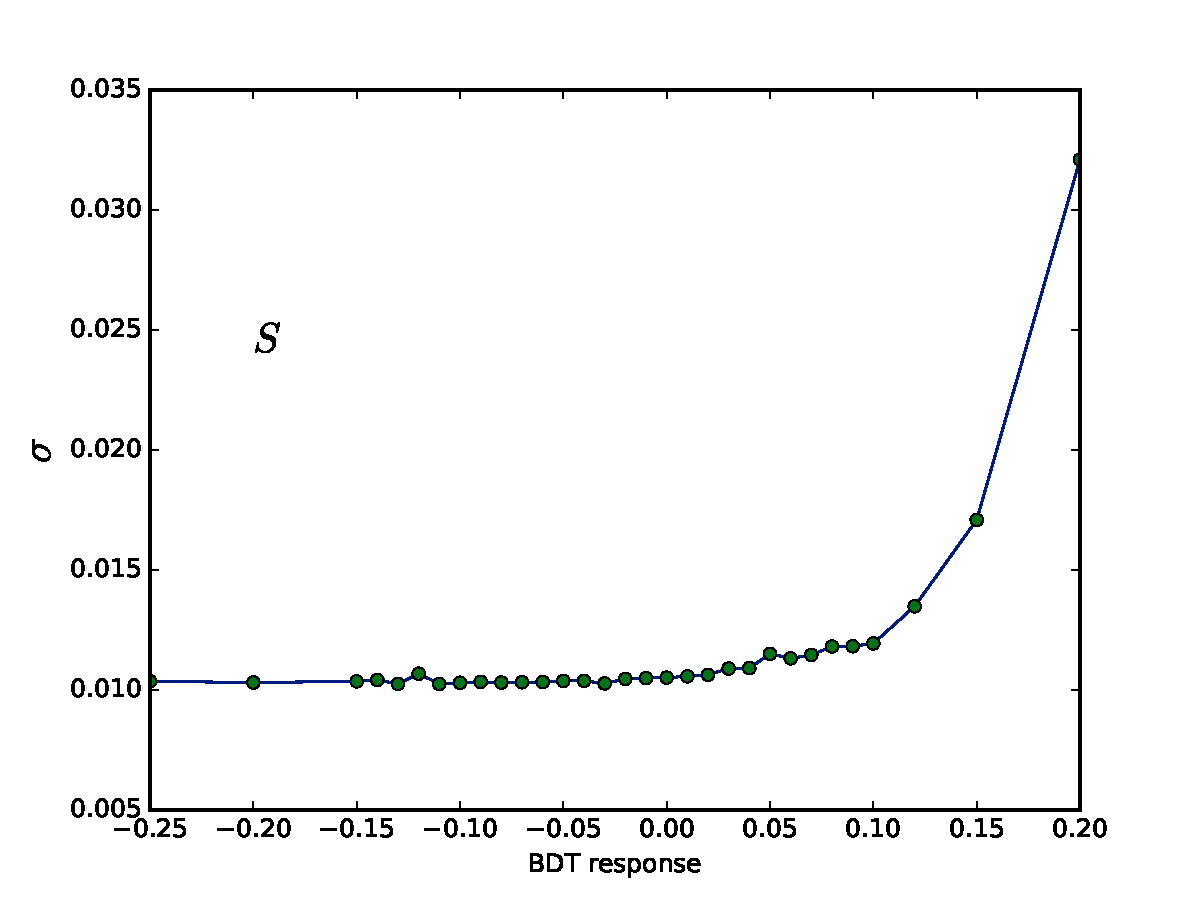
\includegraphics[width=0.45\textwidth]{06selection/figs/sensitiv_Sf.pdf}
    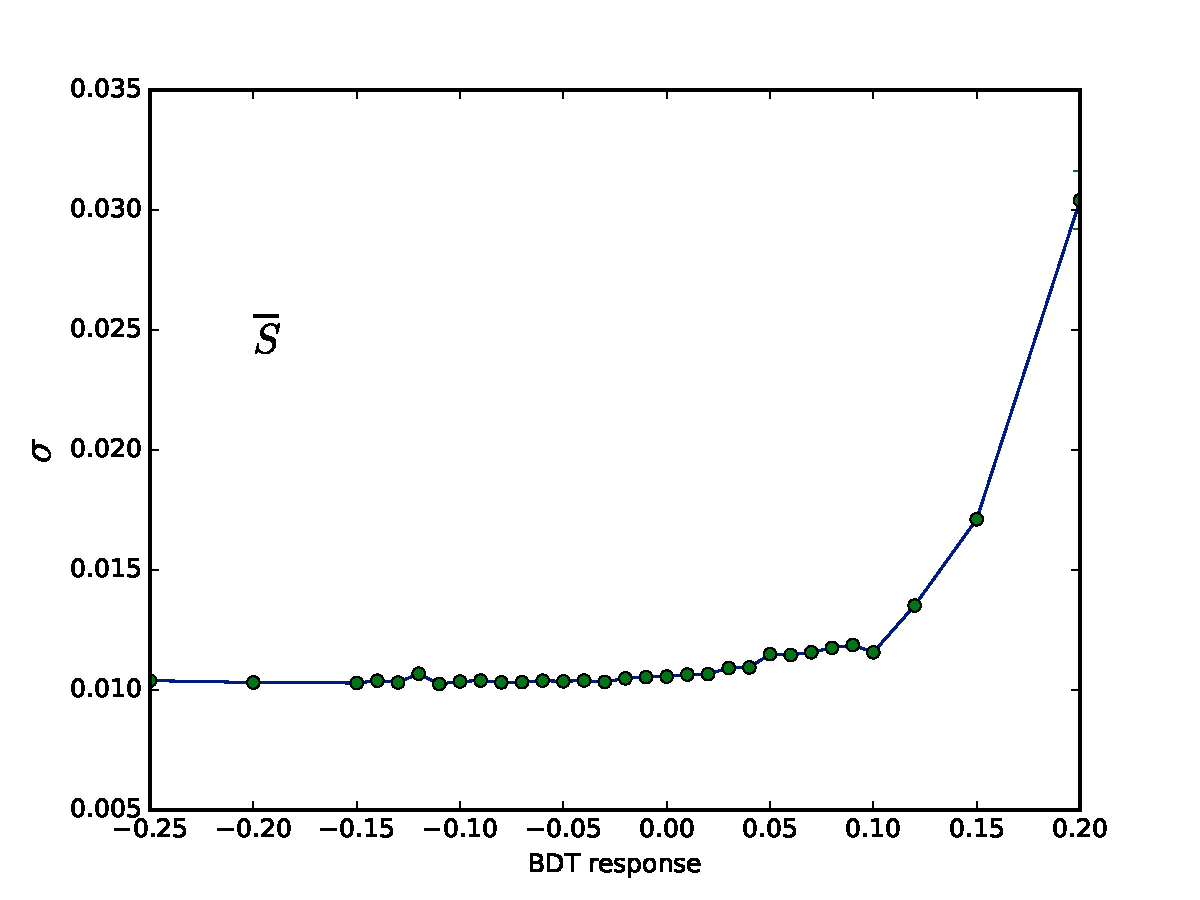
\includegraphics[width=0.45\textwidth]{06selection/figs/sensitiv_Sfbar.pdf}
    \caption{Uncertainty on \Sf (left) and \Sfbar (right) as a function of the \ac{BDT} response.}
    \label{fig:BDTopt}
\end{figure}

\subsection{Multiple Candidates}
\label{sec:MultCands}

Should quote this here:~\cite{Koppenburg:2017zsh}

% - nach Stripping 9% Events haben multiple Kandidaten, entsprechend 18-20% der B Kandidaten teilen ein Event
% - nach Offline Selektion Zahl der Events mit multiplen Kandiadten auf 0.4% runter, und 0.8% der Kandiadten teilen das gleiche Event.
% - im Falle mehrerer PVs wird nun der beste gewählt um konsistent mit Stripping und Trigger zu sein, Events in denen der ursprünglich beste PV nciht mehr da ist, werden entfernt
% - in Anlehnung an Quelle Koppenburg werden alle weiteren verbleibenden Kandidaten als gleich wahrscheinlich Signal eingschätzt und daher wird jeweils ein Kandidate zufällig behalten

\subsection{Selection Performance}
\label{sec:selectionPerformance}

% - Selektions Performanzen wurden bestimmt auf oberem Massenseitenband der 2012 Daten (kombinatorischer Untergrund) und Signal MC für 2012
% - Effizienzen in Tabelle X
% -  Vetos zeigen schlechte Untergrundunterdrückung, da sie nciht kombinatorkik unterdrücken sollen
% - Außerdem wurde als Crosscheck der BDT getrennt nach Jahr und Magnetpolarität auf Daten gecheckt, werte in Tabelle - die absoluten Werte sind nr bedingt aussagekräftig, da Sig+Bkg zu sehen ist. (Vorher noch Polarität am Anfang einführen)
% - Schlussneldich nicht resonanten B->Kpipipi Komponente abgeschätzt mit zwei Strategien:
%   - zunächst Anwendung aller Selektionsschnitte, dann:
%   - erste Methode B-Massenfenster wird ausgeschnitte, anschließend wird die D-Masse für dieses Fenster angesehen - Kombinatorik im D-Massenfenster ist etwa 1% vom Signalpeak - allerdings zeigt D-Massenplot viel mehr Kandidaten??
%   - zweite Methode: In der D-Masse wird der Peak ausgeschnitten, und das B-Massenfenster untersucht (nach Anwendung): Fit einer Exponentialfunktion für kombinatorischen Untergrund und Gaus mit gefixtem Mittelwert, ergibt X Kandidante, Plots zeigen ausgeschnittenens D-Massenfesnster und B-Fit
%   - Verunreinigung durch nicht Resonante untergründe vernachlässigbar
